\documentclass[]{book}
\usepackage{lmodern}
\usepackage{amssymb,amsmath}
\usepackage{ifxetex,ifluatex}
\usepackage{fixltx2e} % provides \textsubscript
\ifnum 0\ifxetex 1\fi\ifluatex 1\fi=0 % if pdftex
  \usepackage[T1]{fontenc}
  \usepackage[utf8]{inputenc}
\else % if luatex or xelatex
  \ifxetex
    \usepackage{mathspec}
  \else
    \usepackage{fontspec}
  \fi
  \defaultfontfeatures{Ligatures=TeX,Scale=MatchLowercase}
\fi
% use upquote if available, for straight quotes in verbatim environments
\IfFileExists{upquote.sty}{\usepackage{upquote}}{}
% use microtype if available
\IfFileExists{microtype.sty}{%
\usepackage{microtype}
\UseMicrotypeSet[protrusion]{basicmath} % disable protrusion for tt fonts
}{}
\usepackage[margin=1in]{geometry}
\usepackage{hyperref}
\hypersetup{unicode=true,
            pdftitle={Introduction to Visualization in R},
            pdfauthor={LTC Melanie Vinton},
            pdfborder={0 0 0},
            breaklinks=true}
\urlstyle{same}  % don't use monospace font for urls
\usepackage{color}
\usepackage{fancyvrb}
\newcommand{\VerbBar}{|}
\newcommand{\VERB}{\Verb[commandchars=\\\{\}]}
\DefineVerbatimEnvironment{Highlighting}{Verbatim}{commandchars=\\\{\}}
% Add ',fontsize=\small' for more characters per line
\usepackage{framed}
\definecolor{shadecolor}{RGB}{248,248,248}
\newenvironment{Shaded}{\begin{snugshade}}{\end{snugshade}}
\newcommand{\KeywordTok}[1]{\textcolor[rgb]{0.13,0.29,0.53}{\textbf{{#1}}}}
\newcommand{\DataTypeTok}[1]{\textcolor[rgb]{0.13,0.29,0.53}{{#1}}}
\newcommand{\DecValTok}[1]{\textcolor[rgb]{0.00,0.00,0.81}{{#1}}}
\newcommand{\BaseNTok}[1]{\textcolor[rgb]{0.00,0.00,0.81}{{#1}}}
\newcommand{\FloatTok}[1]{\textcolor[rgb]{0.00,0.00,0.81}{{#1}}}
\newcommand{\ConstantTok}[1]{\textcolor[rgb]{0.00,0.00,0.00}{{#1}}}
\newcommand{\CharTok}[1]{\textcolor[rgb]{0.31,0.60,0.02}{{#1}}}
\newcommand{\SpecialCharTok}[1]{\textcolor[rgb]{0.00,0.00,0.00}{{#1}}}
\newcommand{\StringTok}[1]{\textcolor[rgb]{0.31,0.60,0.02}{{#1}}}
\newcommand{\VerbatimStringTok}[1]{\textcolor[rgb]{0.31,0.60,0.02}{{#1}}}
\newcommand{\SpecialStringTok}[1]{\textcolor[rgb]{0.31,0.60,0.02}{{#1}}}
\newcommand{\ImportTok}[1]{{#1}}
\newcommand{\CommentTok}[1]{\textcolor[rgb]{0.56,0.35,0.01}{\textit{{#1}}}}
\newcommand{\DocumentationTok}[1]{\textcolor[rgb]{0.56,0.35,0.01}{\textbf{\textit{{#1}}}}}
\newcommand{\AnnotationTok}[1]{\textcolor[rgb]{0.56,0.35,0.01}{\textbf{\textit{{#1}}}}}
\newcommand{\CommentVarTok}[1]{\textcolor[rgb]{0.56,0.35,0.01}{\textbf{\textit{{#1}}}}}
\newcommand{\OtherTok}[1]{\textcolor[rgb]{0.56,0.35,0.01}{{#1}}}
\newcommand{\FunctionTok}[1]{\textcolor[rgb]{0.00,0.00,0.00}{{#1}}}
\newcommand{\VariableTok}[1]{\textcolor[rgb]{0.00,0.00,0.00}{{#1}}}
\newcommand{\ControlFlowTok}[1]{\textcolor[rgb]{0.13,0.29,0.53}{\textbf{{#1}}}}
\newcommand{\OperatorTok}[1]{\textcolor[rgb]{0.81,0.36,0.00}{\textbf{{#1}}}}
\newcommand{\BuiltInTok}[1]{{#1}}
\newcommand{\ExtensionTok}[1]{{#1}}
\newcommand{\PreprocessorTok}[1]{\textcolor[rgb]{0.56,0.35,0.01}{\textit{{#1}}}}
\newcommand{\AttributeTok}[1]{\textcolor[rgb]{0.77,0.63,0.00}{{#1}}}
\newcommand{\RegionMarkerTok}[1]{{#1}}
\newcommand{\InformationTok}[1]{\textcolor[rgb]{0.56,0.35,0.01}{\textbf{\textit{{#1}}}}}
\newcommand{\WarningTok}[1]{\textcolor[rgb]{0.56,0.35,0.01}{\textbf{\textit{{#1}}}}}
\newcommand{\AlertTok}[1]{\textcolor[rgb]{0.94,0.16,0.16}{{#1}}}
\newcommand{\ErrorTok}[1]{\textcolor[rgb]{0.64,0.00,0.00}{\textbf{{#1}}}}
\newcommand{\NormalTok}[1]{{#1}}
\usepackage{longtable,booktabs}
\usepackage{graphicx,grffile}
\makeatletter
\def\maxwidth{\ifdim\Gin@nat@width>\linewidth\linewidth\else\Gin@nat@width\fi}
\def\maxheight{\ifdim\Gin@nat@height>\textheight\textheight\else\Gin@nat@height\fi}
\makeatother
% Scale images if necessary, so that they will not overflow the page
% margins by default, and it is still possible to overwrite the defaults
% using explicit options in \includegraphics[width, height, ...]{}
\setkeys{Gin}{width=\maxwidth,height=\maxheight,keepaspectratio}
\IfFileExists{parskip.sty}{%
\usepackage{parskip}
}{% else
\setlength{\parindent}{0pt}
\setlength{\parskip}{6pt plus 2pt minus 1pt}
}
\setlength{\emergencystretch}{3em}  % prevent overfull lines
\providecommand{\tightlist}{%
  \setlength{\itemsep}{0pt}\setlength{\parskip}{0pt}}
\setcounter{secnumdepth}{5}
% Redefines (sub)paragraphs to behave more like sections
\ifx\paragraph\undefined\else
\let\oldparagraph\paragraph
\renewcommand{\paragraph}[1]{\oldparagraph{#1}\mbox{}}
\fi
\ifx\subparagraph\undefined\else
\let\oldsubparagraph\subparagraph
\renewcommand{\subparagraph}[1]{\oldsubparagraph{#1}\mbox{}}
\fi

%%% Use protect on footnotes to avoid problems with footnotes in titles
\let\rmarkdownfootnote\footnote%
\def\footnote{\protect\rmarkdownfootnote}

%%% Change title format to be more compact
\usepackage{titling}

% Create subtitle command for use in maketitle
\newcommand{\subtitle}[1]{
  \posttitle{
    \begin{center}\large#1\end{center}
    }
}

\setlength{\droptitle}{-2em}
  \title{Introduction to Visualization in R}
  \pretitle{\vspace{\droptitle}\centering\huge}
  \posttitle{\par}
  \author{LTC Melanie Vinton}
  \preauthor{\centering\large\emph}
  \postauthor{\par}
  \predate{\centering\large\emph}
  \postdate{\par}
  \date{2017-10-05}

\usepackage{booktabs}
\usepackage{amsthm}
\makeatletter
\def\thm@space@setup{%
  \thm@preskip=8pt plus 2pt minus 4pt
  \thm@postskip=\thm@preskip
}
\makeatother

\usepackage{amsthm}
\newtheorem{theorem}{Theorem}[chapter]
\newtheorem{lemma}{Lemma}[chapter]
\theoremstyle{definition}
\newtheorem{definition}{Definition}[chapter]
\newtheorem{corollary}{Corollary}[chapter]
\newtheorem{proposition}{Proposition}[chapter]
\theoremstyle{definition}
\newtheorem{example}{Example}[chapter]
\theoremstyle{remark}
\newtheorem*{remark}{Remark}
\begin{document}
\maketitle

{
\setcounter{tocdepth}{1}
\tableofcontents
}
\chapter{Background}\label{background}

This module is an introduction to visualization in R using the ggplot2
package. These relatively simple examples should provide a baseline of
knowledge to allow the user to create far more interesting and
informative graphics than spreadsheet based graphing functionality. Many
of the most impressive visualizations seen today are made in R with
packages like ggplot2.

\chapter{Introduction}\label{introduction}

This module is about creating visualizations in R, using the
\textbf{ggplot2} package. We will add to the basic information about
visualization covered in the pre-course work but continue to focus on
bar charts, line charts, and histograms.

\begin{itemize}
\item
  \textbf{ggplot2} is among the most useful and widely used for
  visualization in R.
\item
  Plots are constructed in layers, which can be more intuitive.
\item
  This package is among the most useful and widely used for
  visualization in R, created by Hadley Wickham.
\item
  There are plotting functions available in base R but \textbf{ggplot2}
  provides a powerful, intuitive framework for creating and customizing
  visualizations.
\end{itemize}

Here's some examples:
\url{http://www.r-graph-gallery.com/portfolio/ggplot2-package}

\section{ggplot2 Package}\label{ggplot2-package}

The \textbf{ggplot2} package is based on the grammar of graphics, which
breaks graphics into parts which are controlled separately and combined.
Every graph has the same basic components - data, a coordinate system,
and geoms that represent data points visually.

First, lets install the packages we will use in this module.

\begin{Shaded}
\begin{Highlighting}[]
\KeywordTok{library}\NormalTok{(ggplot2)}
\KeywordTok{library}\NormalTok{(RColorBrewer)}
\KeywordTok{library}\NormalTok{(plyr)}
\KeywordTok{library}\NormalTok{(dplyr)}
\KeywordTok{library}\NormalTok{(scales)}
\end{Highlighting}
\end{Shaded}

Also, clear your Global Environment.

\begin{Shaded}
\begin{Highlighting}[]
\KeywordTok{rm}\NormalTok{(}\DataTypeTok{list =} \KeywordTok{ls}\NormalTok{())}
\end{Highlighting}
\end{Shaded}

\section{References}\label{references}

Some useful references include:

\begin{itemize}
\item
  \url{http://www.cookbook-r.com}
\item
  \url{http://ggplot2.tidyverse.org/reference/}
\item
  \url{https://www.rstudio.com/resources/cheatsheets/}
\item
  ``R Graphics Cookbook'' by Winston Chang (PDF can be found online at
  \url{http://ase.tufts.edu/bugs/guide/assets/R\%20Graphics\%20Cookbook.pdf})
\item
  \url{http://www.google.com}
\end{itemize}

\section{Layering}\label{layering}

Every graph has the same basic components:

\begin{enumerate}
\def\labelenumi{\arabic{enumi}.}
\tightlist
\item
  Data
\end{enumerate}

\begin{itemize}
\tightlist
\item
  usually a data frame
\end{itemize}

\begin{enumerate}
\def\labelenumi{\arabic{enumi}.}
\setcounter{enumi}{1}
\tightlist
\item
  Aesthetic mapping
\end{enumerate}

\begin{itemize}
\tightlist
\item
  how variables in the data frame map to visual objects on the graph
\item
  objects (or aesthetics) to map to include x-axis, y-axis, size, shape,
  color, transparency
\item
  specified with the \texttt{aes()} function
\end{itemize}

\begin{enumerate}
\def\labelenumi{\arabic{enumi}.}
\setcounter{enumi}{2}
\tightlist
\item
  Geoms that represent data points visually.\\
\end{enumerate}

\begin{itemize}
\tightlist
\item
  specifies the type of plot
\item
  geom = geometric object
\item
  examples (see the cheatsheet!): \texttt{geom\_line()},
  \texttt{geom\_point()}, \texttt{geom\_bar()},
  \texttt{geom\_histogram()}
\end{itemize}

\chapter{Bar Charts}\label{bar-charts}

Bar charts are generally used to display numeric values on the y-axis
for different categories or discrete values on the x-axis. Bar charts
are not well suited for continuous data on the x-axis because try to
make a bar for every possible value of the continuous range.

The heights of the bar on the y-axis can represent counts or values from
your data set. The code for the graphic changes depending on which is
the case.

\section{GDELT Data}\label{gdelt-data}

For the first part of this module we will use the data from the earlier
modules from GDELT, \url{http://www.gdeltproject.com}. The dataframe is
events in Nigeria that involve Chinese actors in January 2017.

If you don't already have it in your environment, open the
``subsahara\_jan17.csv'' file.

\begin{Shaded}
\begin{Highlighting}[]
\NormalTok{subsahara_jan17 <-}\StringTok{ }\KeywordTok{read.csv}\NormalTok{(}\StringTok{"subsahara_jan17.csv"}\NormalTok{)}
\end{Highlighting}
\end{Shaded}

Lets explore the QuadClass variable, which indicates one of four types
of events.

\begin{enumerate}
\def\labelenumi{\arabic{enumi}.}
\item
  Verbal Cooperation
\item
  Material Cooperation
\item
  Verbal Conflict
\item
  Material Conflict
\end{enumerate}

\begin{Shaded}
\begin{Highlighting}[]
\KeywordTok{summary}\NormalTok{(subsahara_jan17$QuadClass)}
\end{Highlighting}
\end{Shaded}

\begin{verbatim}
##    Min. 1st Qu.  Median    Mean 3rd Qu.    Max. 
##   1.000   1.000   1.000   1.523   2.000   4.000
\end{verbatim}

\section{Charts with Counts}\label{charts-with-counts}

Let's create a bar chart the shows the number of events for each level
of the QuadClass variable. First, we start with the \emph{ggplot}
function to define the data and basic aesthetics, in this case which
variable we want to use. Aesthetics can also include visual properties
like size and shape, which we will cover later.

\begin{Shaded}
\begin{Highlighting}[]
\KeywordTok{ggplot}\NormalTok{(}\DataTypeTok{data =} \NormalTok{subsahara_jan17, }\KeywordTok{aes}\NormalTok{(}\DataTypeTok{x =} \NormalTok{QuadClass))}
\end{Highlighting}
\end{Shaded}

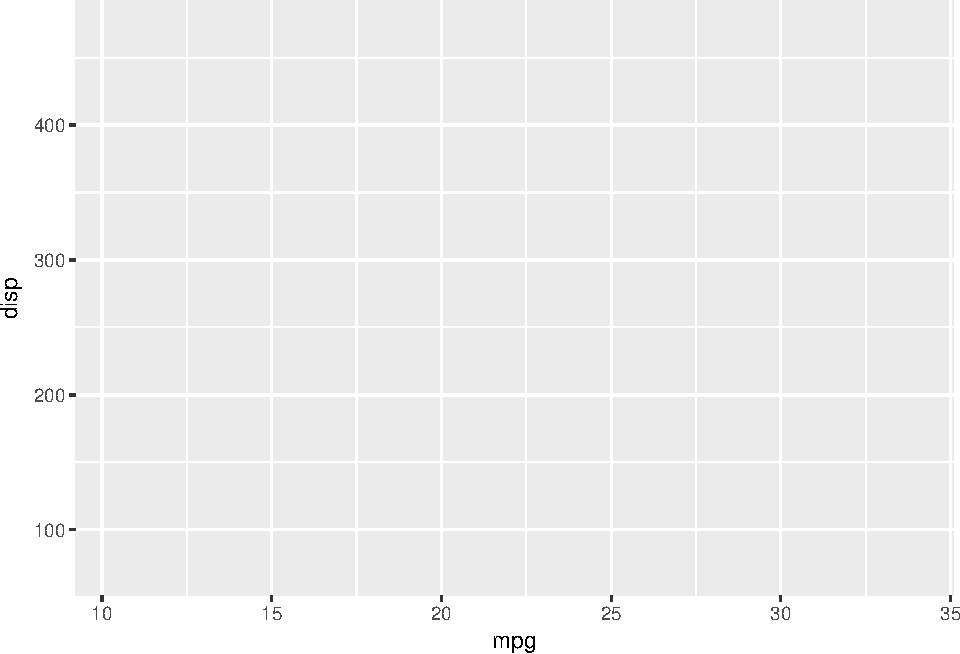
\includegraphics{bookdown-demo_files/figure-latex/unnamed-chunk-5-1.pdf}

Next we need to add a geom function, in this case \emph{geom\_bar()}.
This determines the basic graphical look.

\begin{Shaded}
\begin{Highlighting}[]
\KeywordTok{ggplot}\NormalTok{(}\DataTypeTok{data =} \NormalTok{subsahara_jan17, }\KeywordTok{aes}\NormalTok{(}\DataTypeTok{x =} \NormalTok{QuadClass)) +}
\StringTok{  }\KeywordTok{geom_bar}\NormalTok{()}
\end{Highlighting}
\end{Shaded}

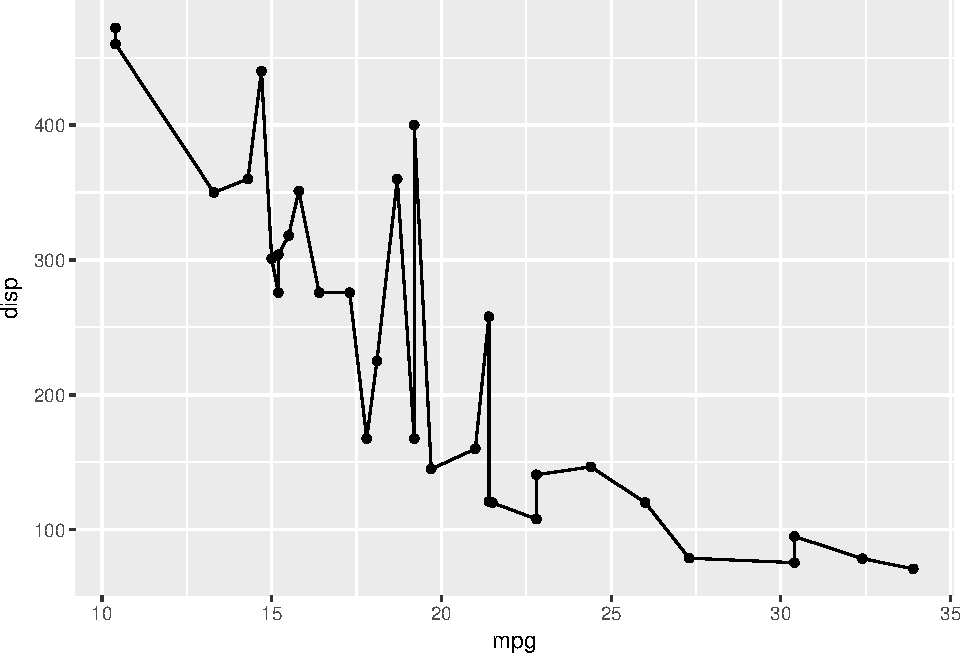
\includegraphics{bookdown-demo_files/figure-latex/unnamed-chunk-7-1.pdf}

\chapter{Change the Look}\label{change-the-look}

Now we want to adjust the look of the chart by applying more aesthetic
controls inside the geom function and using themes and scales.

We will change:

\begin{itemize}
\item
  Color of the bars
\item
  Width of the bars.
\item
  Axis labels.
\item
  Chart title.
\end{itemize}

\section{Colors}\label{colors}

\begin{itemize}
\item
  R has over 600 colors built in which you can refer to by name.
\item
  The \emph{colors()} function provides a list of the names.
\item
  You can also select colors by hexadecimal codes, such as ``\#990000''
  for deep red.
\item
  \href{http://www.cookbook-r.com/Graphs/Colors_(ggplot2)/}{R Cookbook
  Graphs section} has a very useful section on colors and palettes.
\item
  Another good reference for color palettes is
  \url{http://colorbrewer2.org}
\item
  The \emph{RColorBrewer} package provides a set of useful color
  palettes that can be used to customize the color ranges on a graph.
  Use \emph{display.brewer.all()} to see the set of palettes.
\item
  Note: Sometimes you will see the word ``color'' spelled ``colour'' -
  they are interchangeable in R.
\end{itemize}

\section{Changing Bar Colors}\label{changing-bar-colors}

\begin{itemize}
\item
  Change the fill color of the bars with \texttt{fill\ =\ "lightblue"}
\item
  Change the color of the outline of the bars with
  \texttt{color\ =\ "darkblue"}
\item
  Change with width of the bars with \texttt{width\ =\ .5}
\end{itemize}

\begin{Shaded}
\begin{Highlighting}[]
\KeywordTok{ggplot}\NormalTok{(subsahara_jan17, }\KeywordTok{aes}\NormalTok{(}\DataTypeTok{x =} \NormalTok{QuadClass)) +}
\StringTok{  }\KeywordTok{geom_bar}\NormalTok{(}\DataTypeTok{fill =} \StringTok{"lightblue"}\NormalTok{, }\DataTypeTok{color =} \StringTok{"darkblue"}\NormalTok{, }\DataTypeTok{width =} \NormalTok{.}\DecValTok{5}\NormalTok{)}
\end{Highlighting}
\end{Shaded}

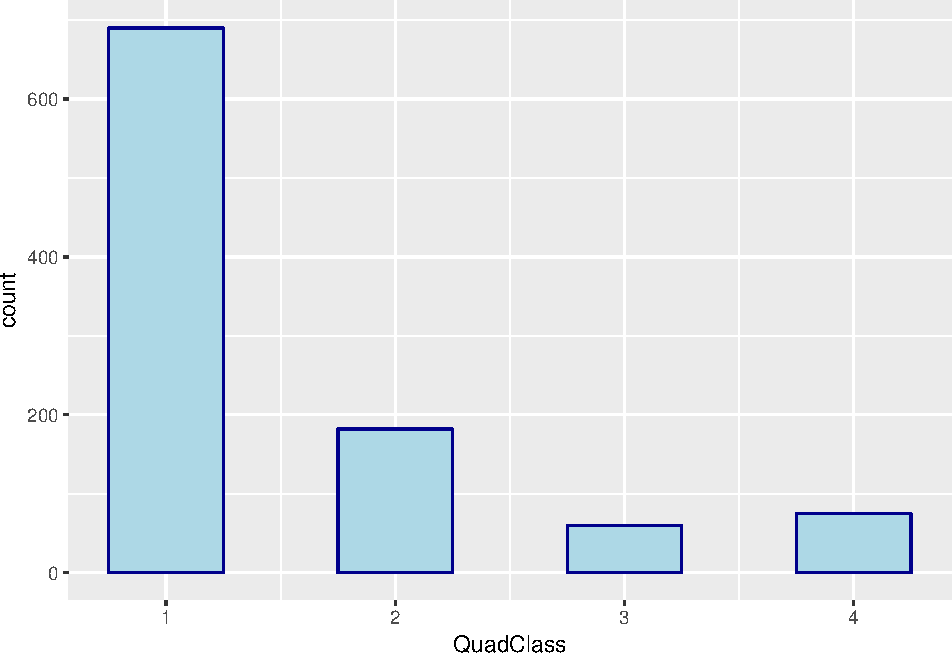
\includegraphics{bookdown-demo_files/figure-latex/unnamed-chunk-9-1.pdf}

\section{Themes}\label{themes}

There are many more options for customizing a graph. Adjusting the look
involves of two different types of elements, themes and scales.

\begin{itemize}
\item
  Theme elements are non-data elements in the plot such as the title,
  legend, and axes.
\item
  To change the appearance of a theme element, use the \emph{theme()}
  function and a corresponding element object.
\item
  Common element objects are text or lines.
\item
  \href{http://ase.tufts.edu/bugs/guide/assets/R\%20Graphics\%20Cookbook.pdf}{R
  Graphics Cookbook} covers this in section 9.4 very clearly.
\end{itemize}

Here's an example, changing the color of the y-axis title to red:

\begin{Shaded}
\begin{Highlighting}[]
\KeywordTok{theme}\NormalTok{(}\DataTypeTok{axis.title.y =} \KeywordTok{element_text}\NormalTok{(}\DataTypeTok{color =} \StringTok{"red"}\NormalTok{))}
\end{Highlighting}
\end{Shaded}

A few other useful theme functions:

\begin{itemize}
\item
  Remove an axis label:
  \texttt{theme(axis.title.x\ =\ element\_blank())}
\item
  Remove grid lines:
  \texttt{theme(panel.grid.major\ =\ element\_blank())}
\item
  Rotate x-axis text labels by 90 degrees:
  \texttt{theme(axis.text.x\ =\ element\_text(angle\ =\ 90))}
\item
  Move the position of a legend:
  \texttt{theme(legend.position\ =\ "bottom")}
\end{itemize}

\section{Scales}\label{scales}

Scale elements map data values to visual values.

\begin{itemize}
\item
  To change the default mapping, a new scale is added.
\item
  The scale function identifies the aesthetic you want to adjust, a
  pre-packaged scale to use, and the specific arguments for what you are
  trying to change.
\item
  Different types of data use different types of aesthetics and scales -
  it is important to match them up correctly.
\item
  The \href{https://www.rstudio.com/resources/cheatsheets}{Data
  Visualization Cheatsheet} are a good reference for different types of
  scales.
\end{itemize}

Here's an example, using \texttt{scale\_x\_reverse()}:

\begin{itemize}
\item
  ``scale'' indicates that we want to customize a data element.
\item
  ``x'' indicates which data element.
\item
  ``reverse'' is used to override the default linear mapping and reverse
  the order on the x-axis.
\end{itemize}

\begin{Shaded}
\begin{Highlighting}[]
\KeywordTok{ggplot}\NormalTok{(subsahara_jan17, }\KeywordTok{aes}\NormalTok{(}\DataTypeTok{x =} \NormalTok{QuadClass)) +}
\StringTok{  }\KeywordTok{geom_bar}\NormalTok{(}\DataTypeTok{fill =} \StringTok{"lightblue"}\NormalTok{,}\DataTypeTok{color =} \StringTok{"darkblue"}\NormalTok{, }\DataTypeTok{width =} \NormalTok{.}\DecValTok{5}\NormalTok{)+}
\StringTok{  }\KeywordTok{scale_x_reverse}\NormalTok{()}
\end{Highlighting}
\end{Shaded}

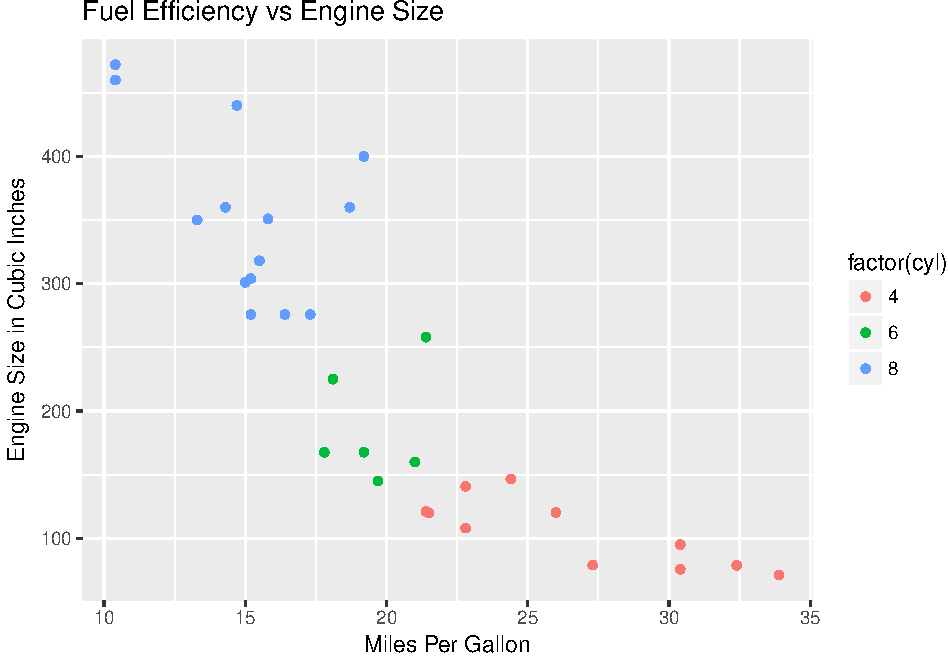
\includegraphics{bookdown-demo_files/figure-latex/unnamed-chunk-11-1.pdf}

\section{Labels and Titles}\label{labels-and-titles}

Going back to our bar chart of the Quad Class varaible, next we will
adjust the labels and add a chart title.

\begin{itemize}
\item
  Change the label on the x-axis with
  \texttt{xlab("Quad\ Class\ of\ Events")}
\item
  Delete the label on the y-axis (currently ``count'') with
  \texttt{theme(axis.title.y\ =\ element\_blank())}
\item
  Add a chart title with
  \texttt{ggtitle("Number\ of\ Events\ by\ Quad\ Class")}
\end{itemize}

\begin{Shaded}
\begin{Highlighting}[]
\KeywordTok{ggplot}\NormalTok{(subsahara_jan17, }\KeywordTok{aes}\NormalTok{(}\DataTypeTok{x =} \NormalTok{QuadClass)) +}
\StringTok{  }\KeywordTok{geom_bar}\NormalTok{(}\DataTypeTok{fill =} \StringTok{"lightblue"}\NormalTok{, }\DataTypeTok{colour =} \StringTok{"darkblue"}\NormalTok{, }\DataTypeTok{width =} \NormalTok{.}\DecValTok{5}\NormalTok{) +}
\StringTok{  }\KeywordTok{xlab}\NormalTok{(}\StringTok{"Quad Class of the Events"}\NormalTok{) +}
\StringTok{  }\KeywordTok{theme}\NormalTok{(}\DataTypeTok{axis.title.y =} \KeywordTok{element_blank}\NormalTok{()) +}
\StringTok{  }\KeywordTok{ggtitle}\NormalTok{(}\StringTok{"Number of Events by Quad Class"}\NormalTok{)}
\end{Highlighting}
\end{Shaded}

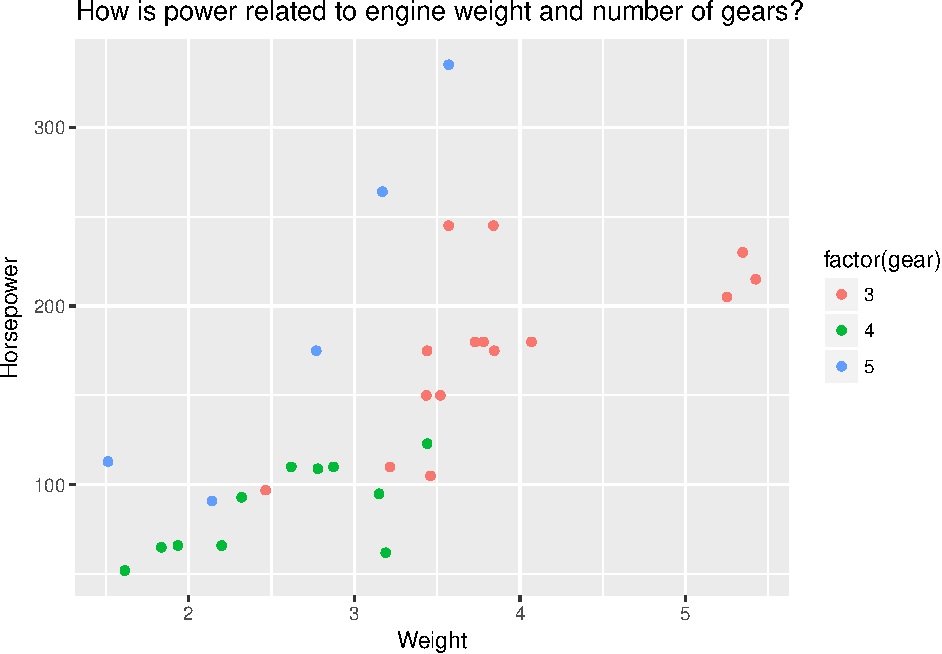
\includegraphics{bookdown-demo_files/figure-latex/unnamed-chunk-12-1.pdf}

\section{Change the Look Exercise}\label{change-the-look-exercise}

\begin{enumerate}
\def\labelenumi{\arabic{enumi}.}
\tightlist
\item
  Change the color of the x-axis label. (hint: use a theme function)
\item
  Increase the size of the chart title. (hint: use a theme function)
\item
  Change the labels on the x-axis to One, Two,Three, and Four. (hint:
  \texttt{scale\_x\_continuous()})
\item
  Change the y-axis label to ``Number of Events''.
\end{enumerate}

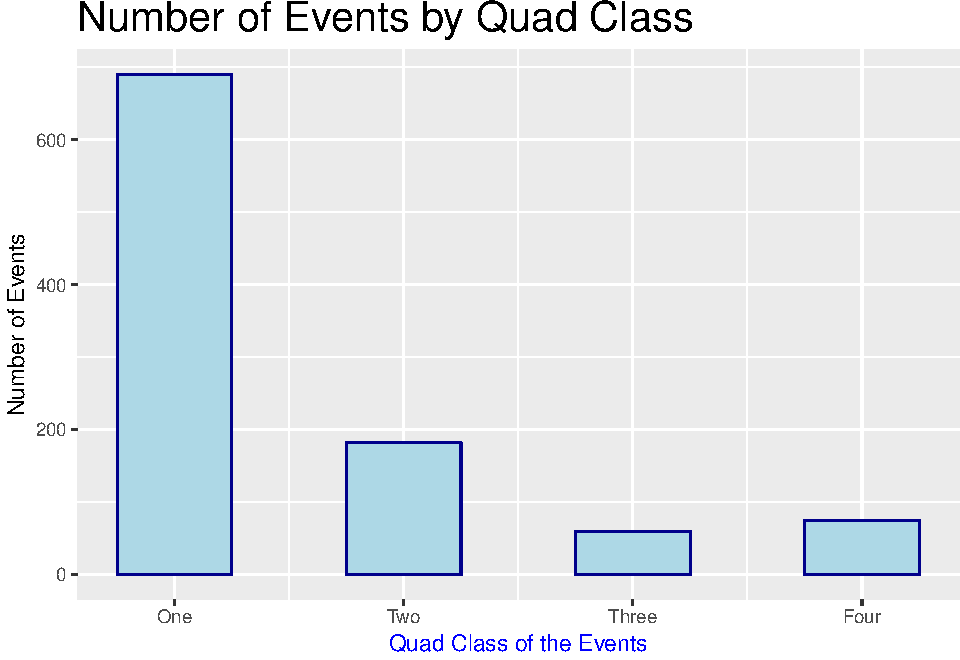
\includegraphics{bookdown-demo_files/figure-latex/unnamed-chunk-13-1.pdf}

\chapter{Bar Charts with Y Values}\label{bar-charts-with-y-values}

Remember that there's a difference in how to make a bar chart with
values from a variable in the data on the y-axis vice counts for a
single variable. The variable used for the y-axis should be continuous.

\section{Values on the Y-axis}\label{values-on-the-y-axis}

We want to get a sense of the tone of articles associated with each Quad
Class. First we need to summarize the data to find the mean of the
AvgTone variable for each QuadClass, using the \emph{summarize} and
\emph{group\_by} functions in \textbf{dplyr}.

\begin{Shaded}
\begin{Highlighting}[]
\NormalTok{quadTone <-}\StringTok{ }\KeywordTok{summarise}\NormalTok{(}\KeywordTok{group_by}\NormalTok{(subsahara_jan17, QuadClass), }\DataTypeTok{meanTone =} \KeywordTok{mean}\NormalTok{(AvgTone))}

\NormalTok{quadTone}
\end{Highlighting}
\end{Shaded}

\begin{verbatim}
## # A tibble: 4 x 2
##   QuadClass   meanTone
##       <int>      <dbl>
## 1         1  1.2619367
## 2         2  1.0109206
## 3         3 -0.8859623
## 4         4 -3.0444109
\end{verbatim}

To chart the new dataframe with values on the y-axis, we must add
\texttt{stat\ =\ "identity"} to the \emph{geom\_bar()} function.

\begin{Shaded}
\begin{Highlighting}[]
\KeywordTok{ggplot}\NormalTok{(quadTone, }\KeywordTok{aes}\NormalTok{(}\DataTypeTok{x =} \NormalTok{QuadClass, }\DataTypeTok{y =} \NormalTok{meanTone)) +}
\StringTok{  }\KeywordTok{geom_bar}\NormalTok{(}\DataTypeTok{stat =} \StringTok{"identity"}\NormalTok{, }\DataTypeTok{width =} \NormalTok{.}\DecValTok{5}\NormalTok{)}
\end{Highlighting}
\end{Shaded}

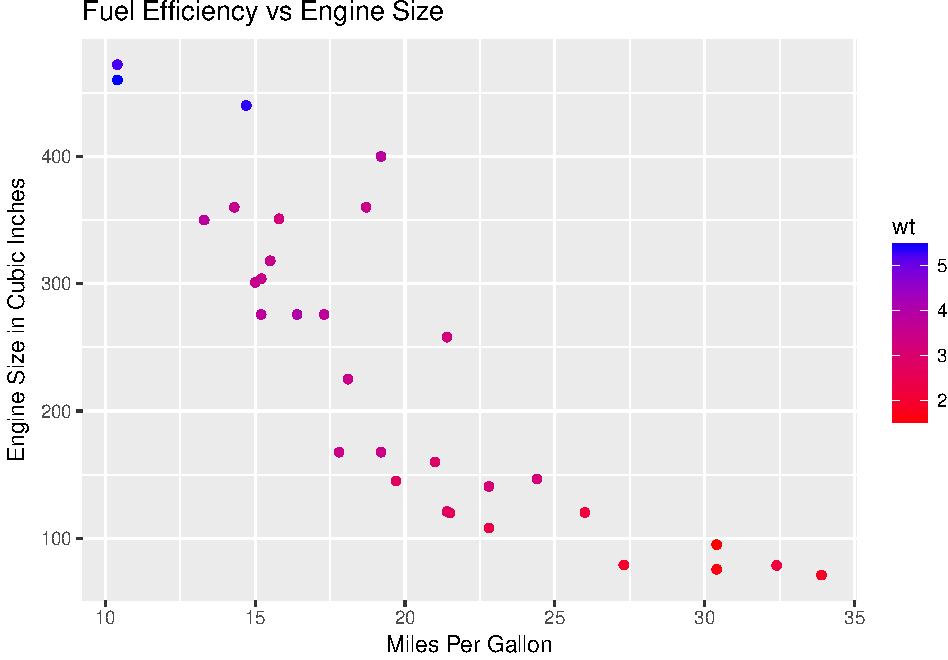
\includegraphics{bookdown-demo_files/figure-latex/unnamed-chunk-16-1.pdf}

\section{Multiple Variables}\label{multiple-variables}

You may want to map multiple variables to the x-axis, to create a
stacked or grouped bar chart where the bars are colored based on the
second variable. In \textbf{ggplot} this is done by adding an aesthetic
mapping called \emph{fill}.

For this we will use a new data set that captures Chinese government
activity in Nigeria, Zambia, and Zimbabwe in the first 2 weeks of
January 2017. If you don't have the ``china\_2weeks'' data in your
environment, then read in the CSV file.

\begin{Shaded}
\begin{Highlighting}[]
\NormalTok{china_2weeks <-}\StringTok{ }\KeywordTok{read.csv}\NormalTok{(}\StringTok{"china_2weeks.csv"}\NormalTok{, }\DataTypeTok{stringsAsFactors =} \OtherTok{FALSE}\NormalTok{)}

\KeywordTok{head}\NormalTok{(china_2weeks)}
\end{Highlighting}
\end{Shaded}

\begin{verbatim}
##         days country n
## 1 2017-01-03      NI 1
## 2 2017-01-03      ZA 0
## 3 2017-01-03      ZI 1
## 4 2017-01-04      NI 0
## 5 2017-01-04      ZA 0
## 6 2017-01-04      ZI 0
\end{verbatim}

\begin{Shaded}
\begin{Highlighting}[]
\KeywordTok{str}\NormalTok{(china_2weeks)}
\end{Highlighting}
\end{Shaded}

\begin{verbatim}
## 'data.frame':    42 obs. of  3 variables:
##  $ days   : chr  "2017-01-03" "2017-01-03" "2017-01-03" "2017-01-04" ...
##  $ country: chr  "NI" "ZA" "ZI" "NI" ...
##  $ n      : int  1 0 1 0 0 0 1 0 0 0 ...
\end{verbatim}

When you look at the variables in the new data set, notice that the
``days'' variable is a Character. This is important to be aware of
because we will have to transform it into a Date later.

To compare the activity of the Chinese government across the same time
period in each of the countries, use these mappings:

\begin{itemize}
\item
  Days on the x-axis.
\item
  Number of events on the y-axis.
\item
  Bars for each of the countries, stacked.
\end{itemize}

\begin{Shaded}
\begin{Highlighting}[]
\KeywordTok{ggplot}\NormalTok{(china_2weeks, }\KeywordTok{aes}\NormalTok{(}\DataTypeTok{x =} \NormalTok{days, }\DataTypeTok{y =} \NormalTok{n, }\DataTypeTok{fill =} \NormalTok{country))+}
\StringTok{  }\KeywordTok{geom_bar}\NormalTok{(}\DataTypeTok{stat =} \StringTok{"identity"}\NormalTok{)}
\end{Highlighting}
\end{Shaded}

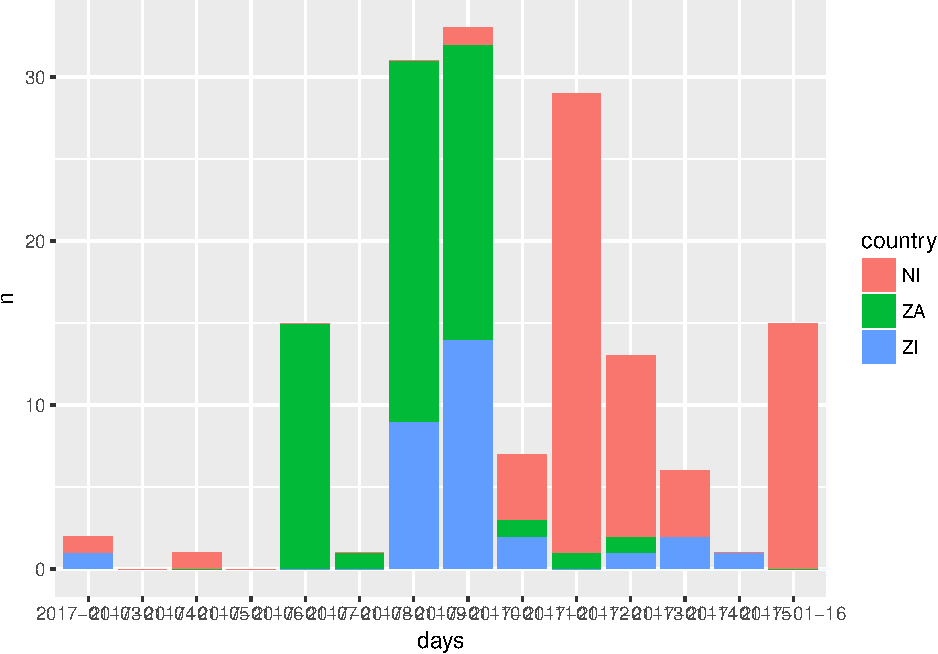
\includegraphics{bookdown-demo_files/figure-latex/unnamed-chunk-18-1.pdf}

\section{Date Sequence}\label{date-sequence}

You can see that this chart needs some formatting to make it more
readable.

\begin{itemize}
\tightlist
\item
  Adjust the labels on the x-axis.

  \begin{itemize}
  \tightlist
  \item
    Create a sequence of dates with the \emph{seq()} function that
    covers every other day in the range of dates in our data.\\
  \item
    That will make the labels easier to read.\\
  \item
    Notice the use of \emph{as.Date()} function.
  \end{itemize}
\end{itemize}

\begin{Shaded}
\begin{Highlighting}[]
\NormalTok{dailybreaks <-}\StringTok{ }\KeywordTok{seq}\NormalTok{(}\KeywordTok{min}\NormalTok{(}\KeywordTok{as.Date}\NormalTok{(china_2weeks$days)),}
                   \KeywordTok{max}\NormalTok{(}\KeywordTok{as.Date}\NormalTok{(china_2weeks$days)),}
                   \DataTypeTok{by=}\StringTok{"2 day"}\NormalTok{)}
\end{Highlighting}
\end{Shaded}

\begin{itemize}
\item
  Use that sequence in a \emph{scale\_x\_date()} function to set the
  date breaks to that sequence.
\item
  Use the \emph{as.Date()} function in the aesthetics for the x-axis to
  make sure the data types match between the data and the scale.
\end{itemize}

\begin{Shaded}
\begin{Highlighting}[]
\KeywordTok{ggplot}\NormalTok{(china_2weeks, }\KeywordTok{aes}\NormalTok{(}\DataTypeTok{x =} \KeywordTok{as.Date}\NormalTok{(days), }\DataTypeTok{y =} \NormalTok{n, }\DataTypeTok{fill =} \NormalTok{country)) +}
\StringTok{  }\KeywordTok{geom_bar}\NormalTok{(}\DataTypeTok{stat =} \StringTok{"identity"}\NormalTok{, }\DataTypeTok{width =} \NormalTok{.}\DecValTok{5}\NormalTok{, }\DataTypeTok{color =} \StringTok{"black"}\NormalTok{) +}
\StringTok{  }\KeywordTok{scale_x_date}\NormalTok{(}\DataTypeTok{breaks =} \NormalTok{dailybreaks)}
\end{Highlighting}
\end{Shaded}

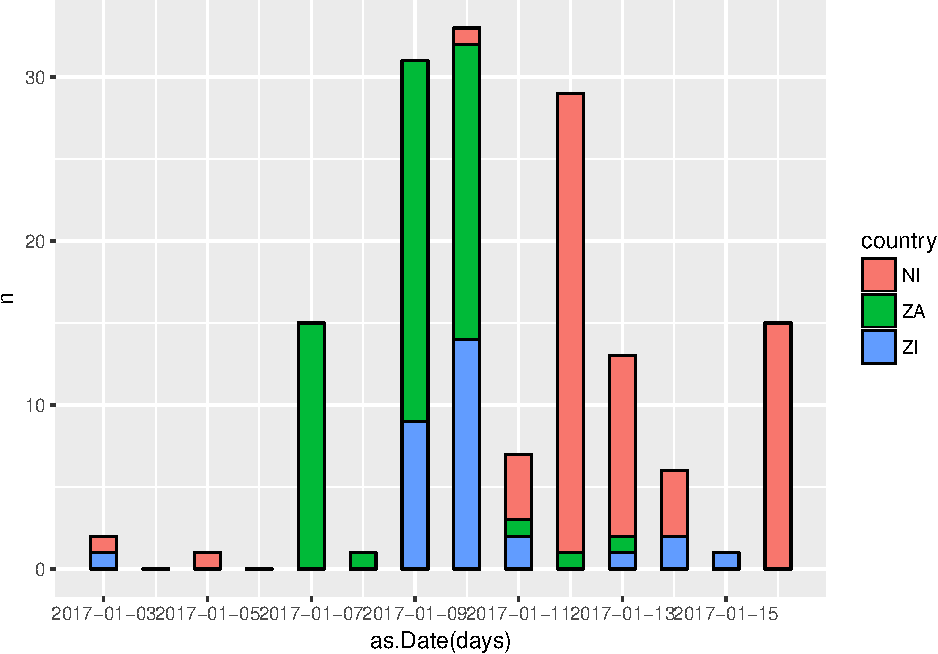
\includegraphics{bookdown-demo_files/figure-latex/unnamed-chunk-20-1.pdf}

\section{hjust and vjust}\label{hjust-and-vjust}

To adjust the position, vertically and horizontally, of text you may
need to use the vjust and hjust commands in conjunction with the angle
command. Note that each command can only take certain values and the
combination results in different positions.

The source of the reference for this is
\url{https://www.r-bloggers.com/hjust-and-vjust/}

\begin{itemize}
\tightlist
\item
  Adjust the angle of the labels on the x-axis with another
  \emph{theme()} function, including the variables:

  \begin{itemize}
  \tightlist
  \item
    \texttt{angle}
  \item
    \texttt{hjust} (horizontal justification)
  \item
    \texttt{vjust} (vertical justification)
  \end{itemize}
\end{itemize}

\begin{Shaded}
\begin{Highlighting}[]
\KeywordTok{ggplot}\NormalTok{(china_2weeks, }\KeywordTok{aes}\NormalTok{(}\DataTypeTok{x =} \KeywordTok{as.Date}\NormalTok{(days), }\DataTypeTok{y =} \NormalTok{n, }\DataTypeTok{fill =} \NormalTok{country)) +}
\StringTok{  }\KeywordTok{geom_bar}\NormalTok{(}\DataTypeTok{stat =} \StringTok{"identity"}\NormalTok{, }\DataTypeTok{width =} \NormalTok{.}\DecValTok{5}\NormalTok{, }\DataTypeTok{color =} \StringTok{"black"}\NormalTok{) +}
\StringTok{  }\KeywordTok{scale_x_date}\NormalTok{(}\DataTypeTok{breaks =} \NormalTok{dailybreaks) +}
\StringTok{  }\KeywordTok{theme}\NormalTok{(}\DataTypeTok{axis.text.x =} \KeywordTok{element_text}\NormalTok{(}\DataTypeTok{angle =} \DecValTok{90}\NormalTok{, }\DataTypeTok{hjust=} \NormalTok{.}\DecValTok{5}\NormalTok{, }\DataTypeTok{vjust=} \NormalTok{.}\DecValTok{5}\NormalTok{))}
\end{Highlighting}
\end{Shaded}

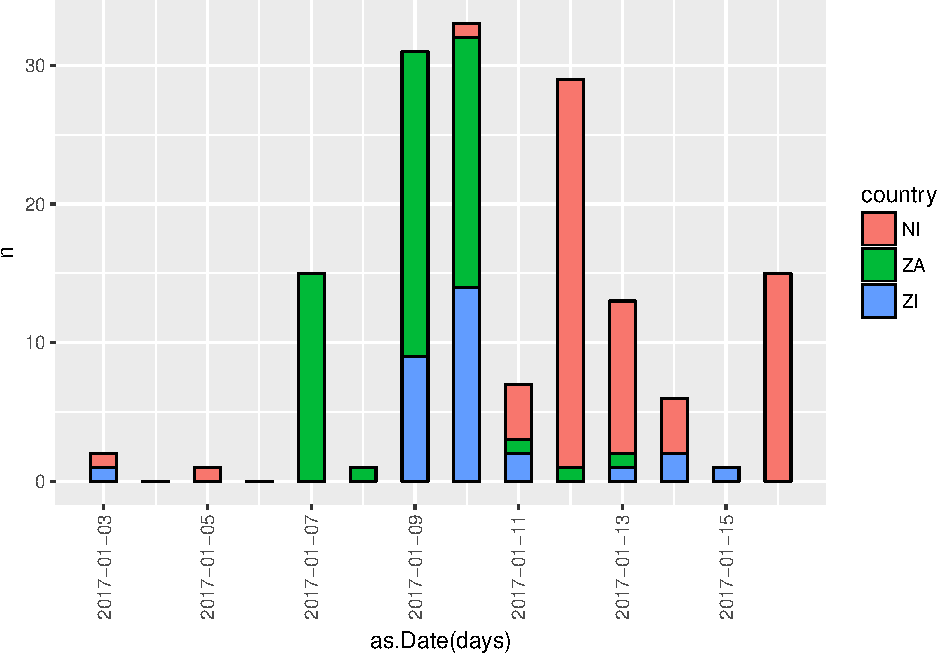
\includegraphics{bookdown-demo_files/figure-latex/unnamed-chunk-21-1.pdf}

\section{Stacked to Grouped Bars}\label{stacked-to-grouped-bars}

\begin{itemize}
\tightlist
\item
  Change from stacked bars to grouped bars that are side by side using
  \texttt{position\ =\ "dodge"} in the \emph{geom\_bar()} function.
\end{itemize}

\begin{Shaded}
\begin{Highlighting}[]
\KeywordTok{ggplot}\NormalTok{(china_2weeks, }\KeywordTok{aes}\NormalTok{(}\DataTypeTok{x =} \KeywordTok{as.Date}\NormalTok{(days), }\DataTypeTok{y =} \NormalTok{n, }\DataTypeTok{fill =} \NormalTok{country)) +}
\StringTok{  }\KeywordTok{geom_bar}\NormalTok{(}\DataTypeTok{stat =} \StringTok{"identity"}\NormalTok{, }\DataTypeTok{width =} \NormalTok{.}\DecValTok{5}\NormalTok{, }\DataTypeTok{color =} \StringTok{"black"}\NormalTok{, }\DataTypeTok{position =} \StringTok{"dodge"}\NormalTok{) +}
\StringTok{  }\KeywordTok{scale_x_date}\NormalTok{(}\DataTypeTok{breaks =} \NormalTok{dailybreaks) +}
\StringTok{  }\KeywordTok{theme}\NormalTok{(}\DataTypeTok{axis.text.x =} \KeywordTok{element_text}\NormalTok{(}\DataTypeTok{angle =} \DecValTok{90}\NormalTok{, }\DataTypeTok{hjust=} \NormalTok{.}\DecValTok{5}\NormalTok{, }\DataTypeTok{vjust=} \NormalTok{.}\DecValTok{5}\NormalTok{))}
\end{Highlighting}
\end{Shaded}

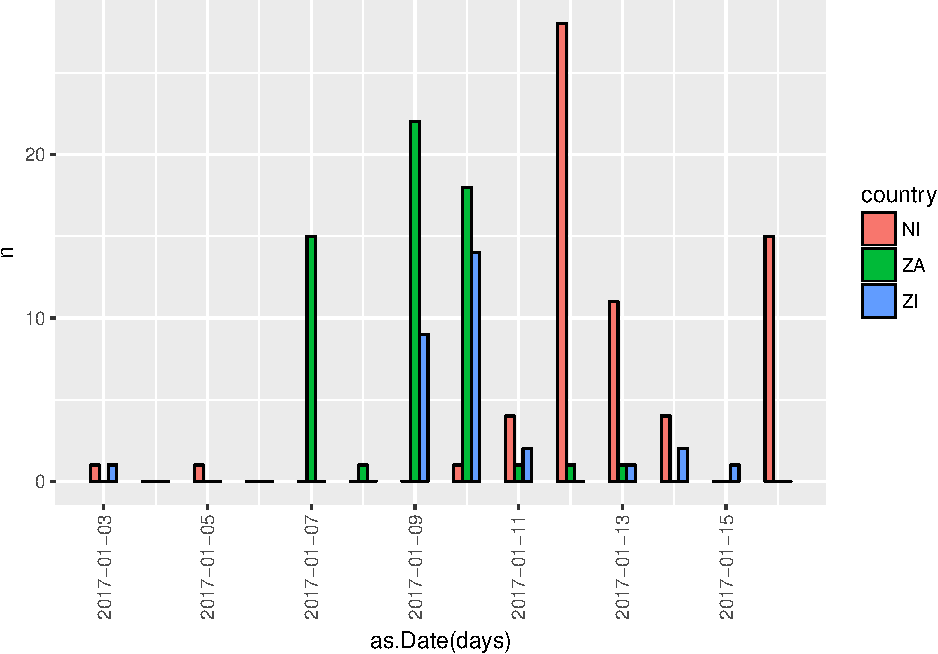
\includegraphics{bookdown-demo_files/figure-latex/unnamed-chunk-22-1.pdf}

\section{Legends}\label{legends}

We want to make some changes to the legend on our chart.

\begin{itemize}
\item
  The legend position is controlled by the \emph{theme()} function:
  \texttt{theme(legend.position\ =\ "bottom")}
\item
  Change the legend title with \texttt{labs(fill\ =\ "Country\ Name")}
\item
  Change the text of the labels with
  \texttt{scale\_fill\_discrete(labels\ =\ c("Nigeria","Zambia","Zimbabwe"))}
\item
  Remove the x-axis label and change the y-axis label.
\end{itemize}

\begin{Shaded}
\begin{Highlighting}[]
\KeywordTok{ggplot}\NormalTok{(china_2weeks, }\KeywordTok{aes}\NormalTok{(}\DataTypeTok{x =} \KeywordTok{as.Date}\NormalTok{(days), }\DataTypeTok{y =} \NormalTok{n, }\DataTypeTok{fill =} \NormalTok{country))+}
\StringTok{  }\KeywordTok{geom_bar}\NormalTok{(}\DataTypeTok{stat =} \StringTok{"identity"}\NormalTok{, }\DataTypeTok{position =} \StringTok{"dodge"}\NormalTok{, }\DataTypeTok{width =} \NormalTok{.}\DecValTok{5}\NormalTok{, }\DataTypeTok{color =} \StringTok{"black"}\NormalTok{)+}
\StringTok{  }\KeywordTok{scale_x_date}\NormalTok{(}\DataTypeTok{breaks =} \NormalTok{dailybreaks) +}
\StringTok{  }\KeywordTok{theme}\NormalTok{(}\DataTypeTok{axis.text.x =} \KeywordTok{element_text}\NormalTok{(}\DataTypeTok{angle =} \DecValTok{90}\NormalTok{, }\DataTypeTok{hjust=} \NormalTok{.}\DecValTok{5}\NormalTok{, }\DataTypeTok{vjust=} \NormalTok{.}\DecValTok{5}\NormalTok{)) +}
\StringTok{  }\KeywordTok{theme}\NormalTok{(}\DataTypeTok{axis.title.x =} \KeywordTok{element_blank}\NormalTok{()) +}
\StringTok{  }\KeywordTok{ylab}\NormalTok{(}\StringTok{"Number of Events"}\NormalTok{) +}
\StringTok{  }\KeywordTok{theme}\NormalTok{(}\DataTypeTok{legend.position =} \StringTok{"bottom"}\NormalTok{)+}
\StringTok{  }\KeywordTok{labs}\NormalTok{(}\DataTypeTok{fill =} \StringTok{"Country Name"}\NormalTok{) +}
\StringTok{  }\KeywordTok{scale_fill_discrete}\NormalTok{(}\DataTypeTok{labels =} \KeywordTok{c}\NormalTok{(}\StringTok{"Nigeria"}\NormalTok{,}\StringTok{"Zambia"}\NormalTok{,}\StringTok{"Zimbabwe"}\NormalTok{))}
\end{Highlighting}
\end{Shaded}

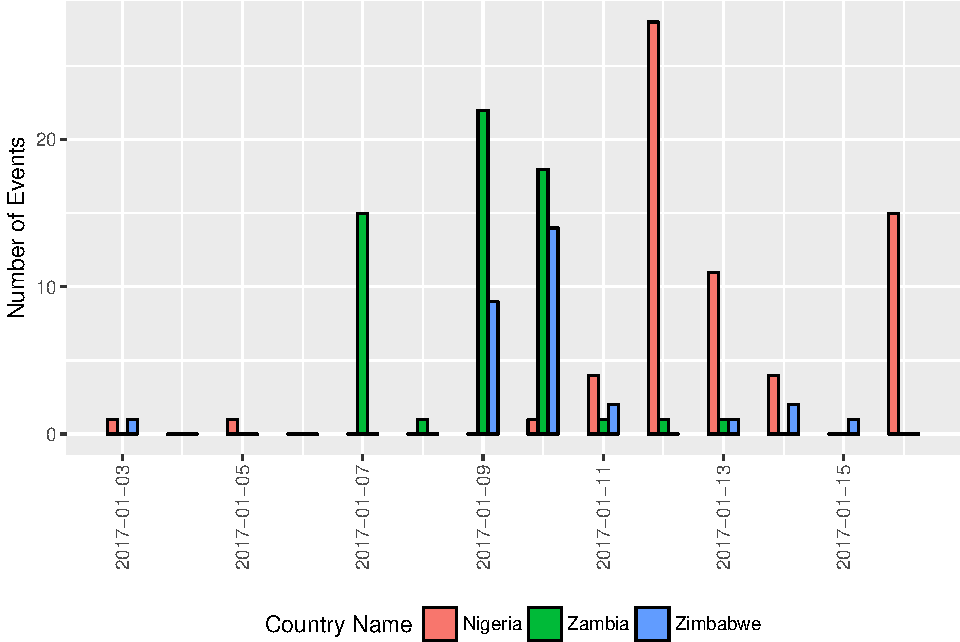
\includegraphics{bookdown-demo_files/figure-latex/unnamed-chunk-23-1.pdf}

\section{Color Palette}\label{color-palette}

The colors used for each bar are based on a default color palette which
can be changed.

Remember this reference:
\url{http://www.cookbook-r.com/Graphs/Colors_(ggplot2)/}

The \textbf{RColorBrewer} package offeres pre-defined color scales.

\begin{itemize}
\item
  Use \emph{display.brewer.all()} to see the set of palettes.
\item
  To use the RColorBrewer palettes, you need to use the
  \texttt{scale\_fill\_brewer()} function as the scale for the ``fill''
  variable, instead of \texttt{scale\_fill\_discrete()}.
\item
  Include the parameters for ``palette'' and ``labels''.
\item
  See section 12.3 in the ``R Graphics Cookbook''.
\end{itemize}

Change the color palette of the bars with
\texttt{scale\_fill\_brewer(palette\ =\ "YlOrRd",\ labels\ =\ c("Nigeria","Zambia","Zimbabwe"))}

\begin{Shaded}
\begin{Highlighting}[]
\KeywordTok{ggplot}\NormalTok{(china_2weeks, }\KeywordTok{aes}\NormalTok{(}\DataTypeTok{x =} \KeywordTok{as.Date}\NormalTok{(days), }\DataTypeTok{y =} \NormalTok{n, }\DataTypeTok{fill =} \NormalTok{country))+}
\StringTok{  }\KeywordTok{geom_bar}\NormalTok{(}\DataTypeTok{stat =} \StringTok{"identity"}\NormalTok{, }\DataTypeTok{position =} \StringTok{"dodge"}\NormalTok{, }\DataTypeTok{width =} \NormalTok{.}\DecValTok{5}\NormalTok{, }\DataTypeTok{color =} \StringTok{"black"}\NormalTok{)+}
\StringTok{  }\KeywordTok{scale_x_date}\NormalTok{(}\DataTypeTok{breaks =} \NormalTok{dailybreaks) +}
\StringTok{  }\KeywordTok{theme}\NormalTok{(}\DataTypeTok{axis.text.x =} \KeywordTok{element_text}\NormalTok{(}\DataTypeTok{angle =} \DecValTok{90}\NormalTok{, }\DataTypeTok{hjust=} \NormalTok{.}\DecValTok{5}\NormalTok{, }\DataTypeTok{vjust=} \NormalTok{.}\DecValTok{5}\NormalTok{)) +}
\StringTok{  }\KeywordTok{theme}\NormalTok{(}\DataTypeTok{axis.title.x =} \KeywordTok{element_blank}\NormalTok{()) +}
\StringTok{  }\KeywordTok{ylab}\NormalTok{(}\StringTok{"Number of Events"}\NormalTok{) +}
\StringTok{  }\KeywordTok{theme}\NormalTok{(}\DataTypeTok{legend.position =} \StringTok{"bottom"}\NormalTok{)+}
\StringTok{  }\KeywordTok{labs}\NormalTok{(}\DataTypeTok{fill =} \StringTok{"Country Name"}\NormalTok{) +}
\StringTok{  }\KeywordTok{scale_fill_brewer}\NormalTok{(}\DataTypeTok{palette =} \StringTok{"YlOrRd"}\NormalTok{,}\DataTypeTok{labels =} \KeywordTok{c}\NormalTok{(}\StringTok{"Nigeria"}\NormalTok{,}\StringTok{"Zambia"}\NormalTok{,}\StringTok{"Zimbabwe"}\NormalTok{))}
\end{Highlighting}
\end{Shaded}

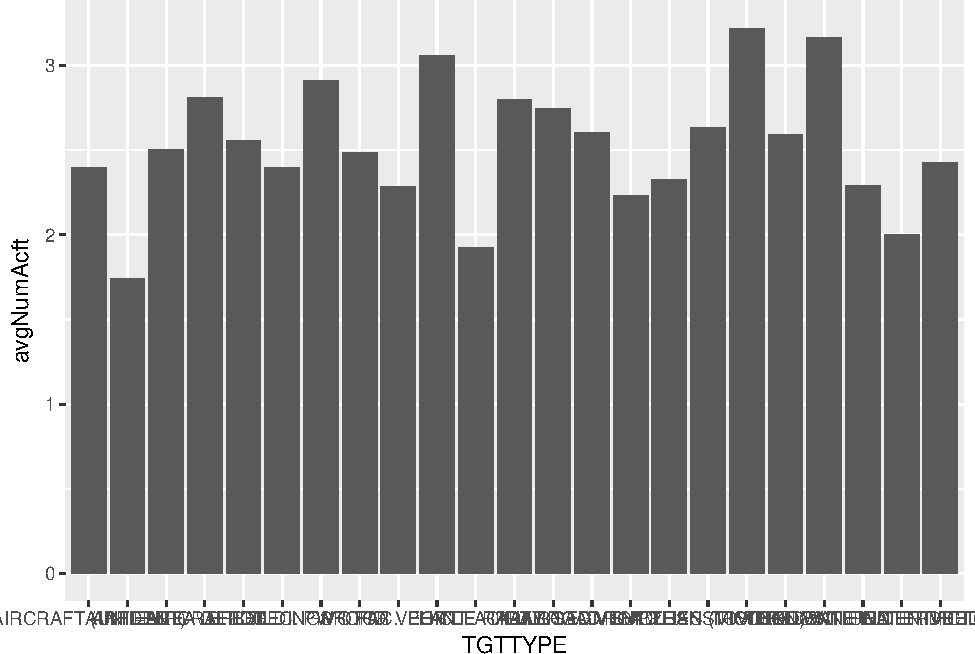
\includegraphics{bookdown-demo_files/figure-latex/unnamed-chunk-24-1.pdf}

\chapter{Line Charts}\label{line-charts}

Line charts are typically used when all variable are continuous. Often,
line charts are better for graphics involving dates and/or times (often
called time series charts) because trends are more visible.

Let's create some simple time series data with the ``china\_2weeks''
dataframe.

\begin{Shaded}
\begin{Highlighting}[]
\NormalTok{china_all <-}\StringTok{ }\KeywordTok{summarize}\NormalTok{(}\KeywordTok{group_by}\NormalTok{(china_2weeks, days), }\DataTypeTok{total =} \KeywordTok{sum}\NormalTok{(n))}
\NormalTok{china_all$days <-}\StringTok{ }\KeywordTok{as.Date}\NormalTok{(china_all$days)}
\end{Highlighting}
\end{Shaded}

Notice that there are no dates that are skipped - we have data for every
day. That's great because it means we don't need to fill in the gaps.

\section{Basic Line Charts}\label{basic-line-charts}

In \textbf{ggplot}, line charts use geom function \emph{geom\_line()}.

Let's create a plot of the total events by day.

\begin{Shaded}
\begin{Highlighting}[]
\KeywordTok{ggplot}\NormalTok{(china_all, }\KeywordTok{aes}\NormalTok{(}\DataTypeTok{x =} \NormalTok{days, }\DataTypeTok{y =} \NormalTok{total))+}
\StringTok{  }\KeywordTok{geom_line}\NormalTok{()}
\end{Highlighting}
\end{Shaded}

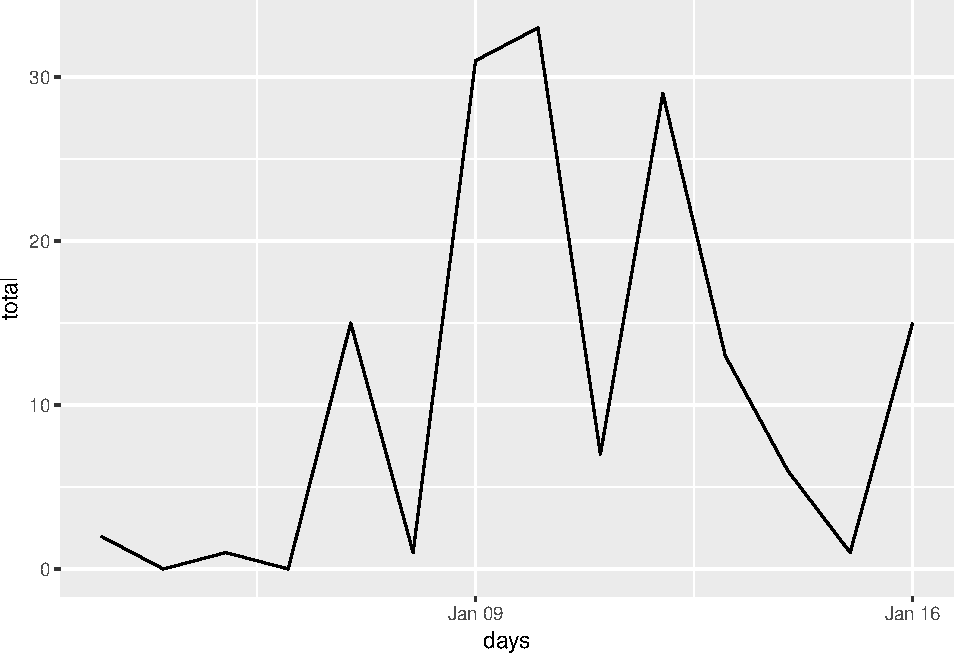
\includegraphics{bookdown-demo_files/figure-latex/unnamed-chunk-27-1.pdf}

\section{Multi-Variable Line Charts}\label{multi-variable-line-charts}

You can also plot multiple lines on a chart. We will use the
china\_2weeks dataframe and plot a line for each country.

\begin{itemize}
\item
  To change the color of the line based on country, we need to change
  the \texttt{fill} aesthetic to \texttt{color}.
\item
  You must have another aesthetic besides x and y so that \emph{ggplot}
  knows how to group the data.
\end{itemize}

\begin{Shaded}
\begin{Highlighting}[]
\KeywordTok{ggplot}\NormalTok{(china_2weeks, }\KeywordTok{aes}\NormalTok{(}\DataTypeTok{x =} \KeywordTok{as.Date}\NormalTok{(days), }\DataTypeTok{y =} \NormalTok{n, }\DataTypeTok{color =} \NormalTok{country))+}
\StringTok{  }\KeywordTok{geom_line}\NormalTok{()}
\end{Highlighting}
\end{Shaded}

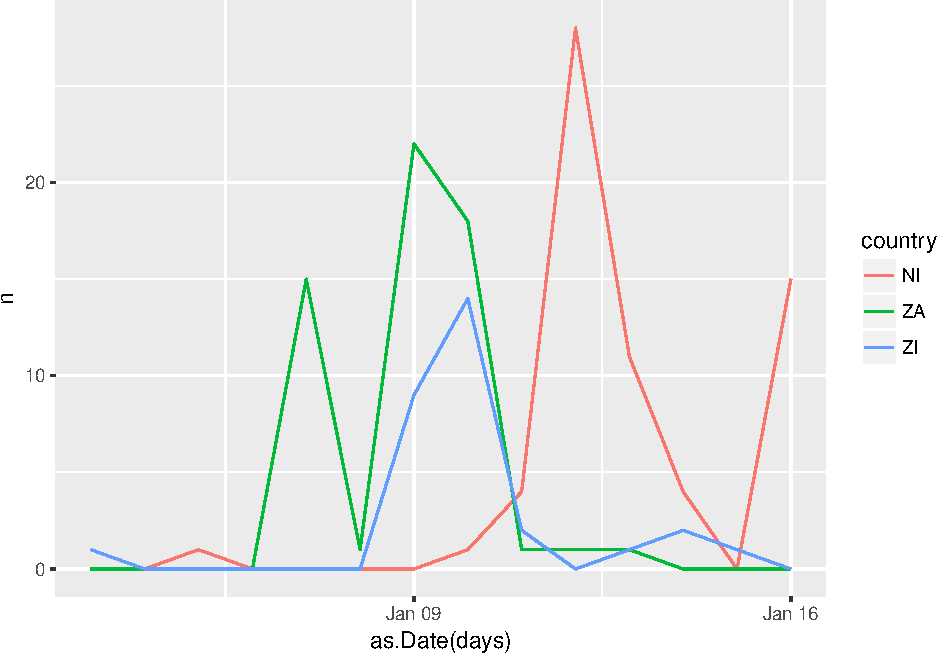
\includegraphics{bookdown-demo_files/figure-latex/unnamed-chunk-28-1.pdf}

\section{Adjust the Look}\label{adjust-the-look}

We can make some adjustments to the look of the line chart.

A good reference for points and lines:
\url{http://www.cookbook-r.com/Graphs/Shapes_and_line_types/}

\begin{itemize}
\item
  Map the country to line type instead of color with
  \texttt{linetype\ =\ country}
\item
  Increase the width of the line with \texttt{geom\_line(size\ =\ 1)}
\item
  Add points and change the shape and size of the point with
  \texttt{geom\_point(shape\ =\ 15,\ size\ =\ 2)}
\end{itemize}

\begin{Shaded}
\begin{Highlighting}[]
\KeywordTok{ggplot}\NormalTok{(china_2weeks, }\KeywordTok{aes}\NormalTok{(}\DataTypeTok{x =} \KeywordTok{as.Date}\NormalTok{(days), }\DataTypeTok{y =} \NormalTok{n, }\DataTypeTok{linetype =} \NormalTok{country))+}
\StringTok{  }\KeywordTok{geom_line}\NormalTok{(}\DataTypeTok{size =} \DecValTok{1}\NormalTok{) +}
\StringTok{  }\KeywordTok{geom_point}\NormalTok{(}\DataTypeTok{shape =} \DecValTok{15}\NormalTok{, }\DataTypeTok{size =} \DecValTok{2}\NormalTok{)}
\end{Highlighting}
\end{Shaded}

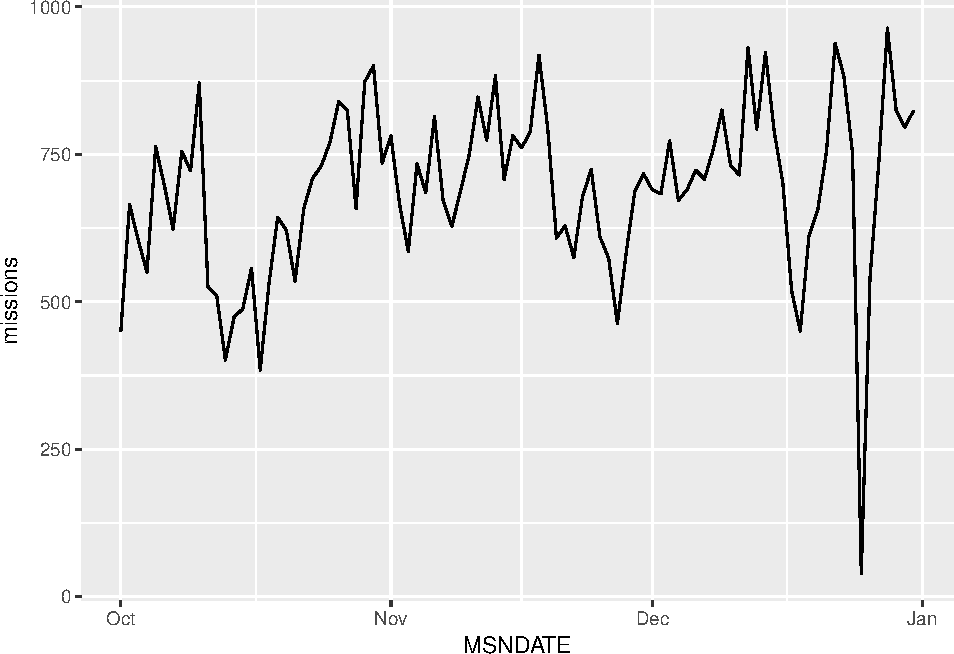
\includegraphics{bookdown-demo_files/figure-latex/unnamed-chunk-29-1.pdf}

\chapter{Histograms}\label{histograms}

A histogram is used to map a continuous variable to the x-axis and use
bins to depict the distribution of that variable.

\begin{itemize}
\item
  In \textbf{ggplot}, histograms use geom function
  \emph{geom\_histogram()}.
\item
  In the subsahara\_jan17 dataset, a continuous variable is NumMentions,
  which is the number of mentions of the event across all source
  documents, an indicator of the importance of the event.
\item
  We want to see the distribution of the NumMentions variable.
\end{itemize}

\begin{Shaded}
\begin{Highlighting}[]
\KeywordTok{ggplot}\NormalTok{(subsahara_jan17, }\KeywordTok{aes}\NormalTok{(}\DataTypeTok{x=}\NormalTok{NumMentions))+}
\StringTok{  }\KeywordTok{geom_histogram}\NormalTok{()}
\end{Highlighting}
\end{Shaded}

\begin{verbatim}
FALSE `stat_bin()` using `bins = 30`. Pick better value with `binwidth`.
\end{verbatim}

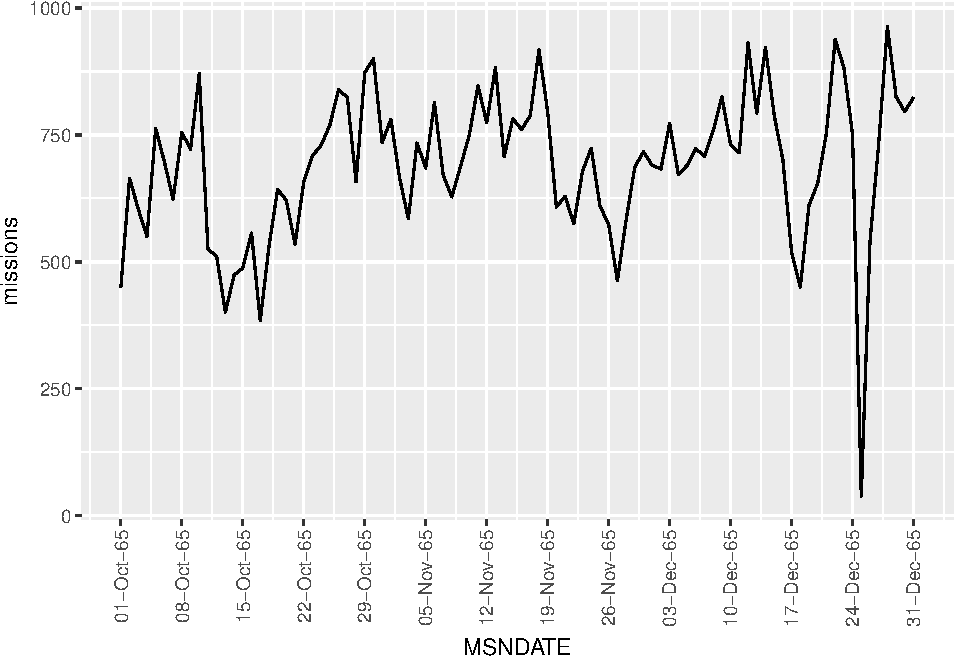
\includegraphics{bookdown-demo_files/figure-latex/unnamed-chunk-31-1.pdf}

The default in \textbf{ggplot} is 30 bins. But we can set the number of
bins in two ways. First we want to find the max and min of the variable.

\begin{Shaded}
\begin{Highlighting}[]
\KeywordTok{summary}\NormalTok{(subsahara_jan17$NumMentions)}
\end{Highlighting}
\end{Shaded}

\begin{verbatim}
##    Min. 1st Qu.  Median    Mean 3rd Qu.    Max. 
##   1.000   2.000   2.000   3.372   4.000  17.000
\end{verbatim}

To set the width of the bins use \texttt{binwidth\ =\ 2} This will
create bins from 1 up to but not including 3, 3 up to but not including
5, and so on.

\begin{Shaded}
\begin{Highlighting}[]
\KeywordTok{ggplot}\NormalTok{(subsahara_jan17, }\KeywordTok{aes}\NormalTok{(}\DataTypeTok{x =} \NormalTok{NumMentions)) +}
\StringTok{  }\KeywordTok{geom_histogram}\NormalTok{(}\DataTypeTok{binwidth =} \DecValTok{2}\NormalTok{, }\DataTypeTok{fill =} \StringTok{"lightblue"}\NormalTok{, }\DataTypeTok{color =} \StringTok{"black"}\NormalTok{)}
\end{Highlighting}
\end{Shaded}

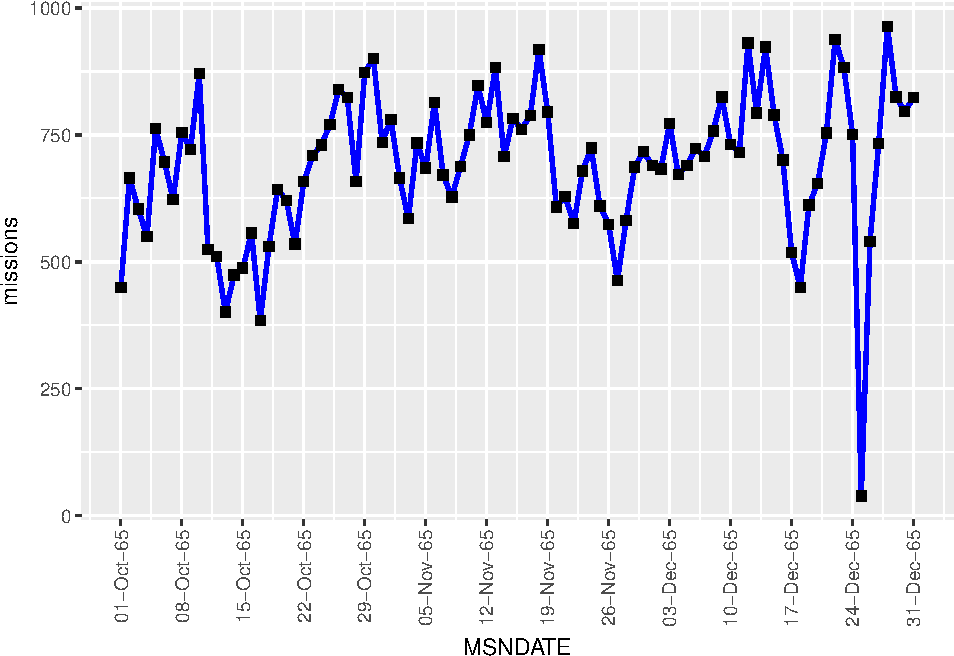
\includegraphics{bookdown-demo_files/figure-latex/unnamed-chunk-33-1.pdf}

To set the number of bins use \texttt{bins\ =\ 5}

\begin{Shaded}
\begin{Highlighting}[]
\KeywordTok{ggplot}\NormalTok{(subsahara_jan17, }\KeywordTok{aes}\NormalTok{(}\DataTypeTok{x =} \NormalTok{NumMentions)) +}
\StringTok{  }\KeywordTok{geom_histogram}\NormalTok{(}\DataTypeTok{bins =}\DecValTok{5}\NormalTok{, }\DataTypeTok{fill =} \StringTok{"lightblue"}\NormalTok{, }\DataTypeTok{color =} \StringTok{"black"}\NormalTok{)}
\end{Highlighting}
\end{Shaded}

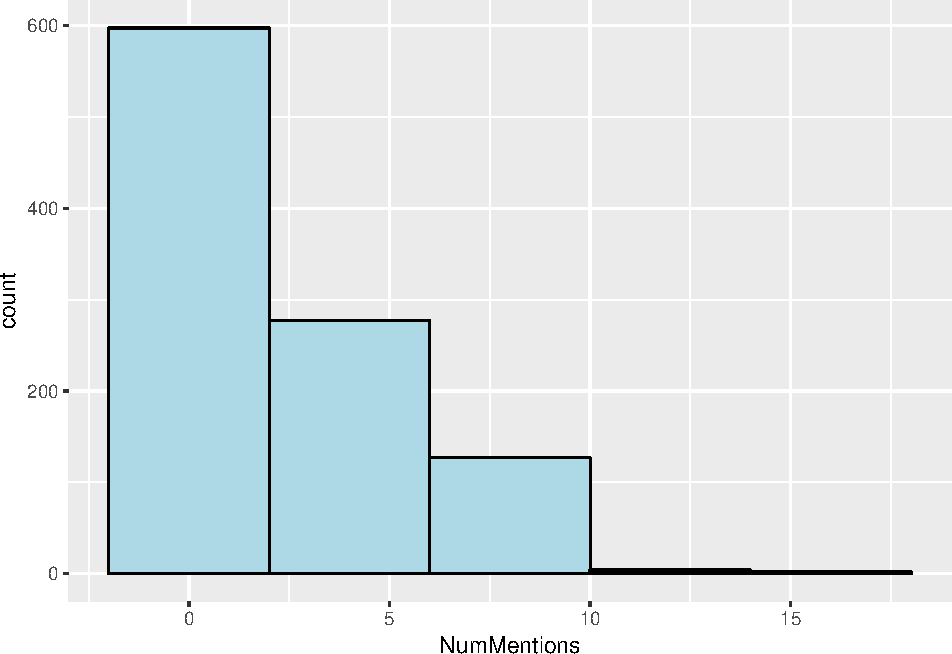
\includegraphics{bookdown-demo_files/figure-latex/unnamed-chunk-34-1.pdf}

\chapter{Practical Exercise}\label{practical-exercise}

Try to recreate the following charts. Use the ``subsahara\_jan17.csv''
data.

\section{Bar: Count of Events by Event Base
Code}\label{bar-count-of-events-by-event-base-code}

Hint: convert EventBaseCode to a factor.

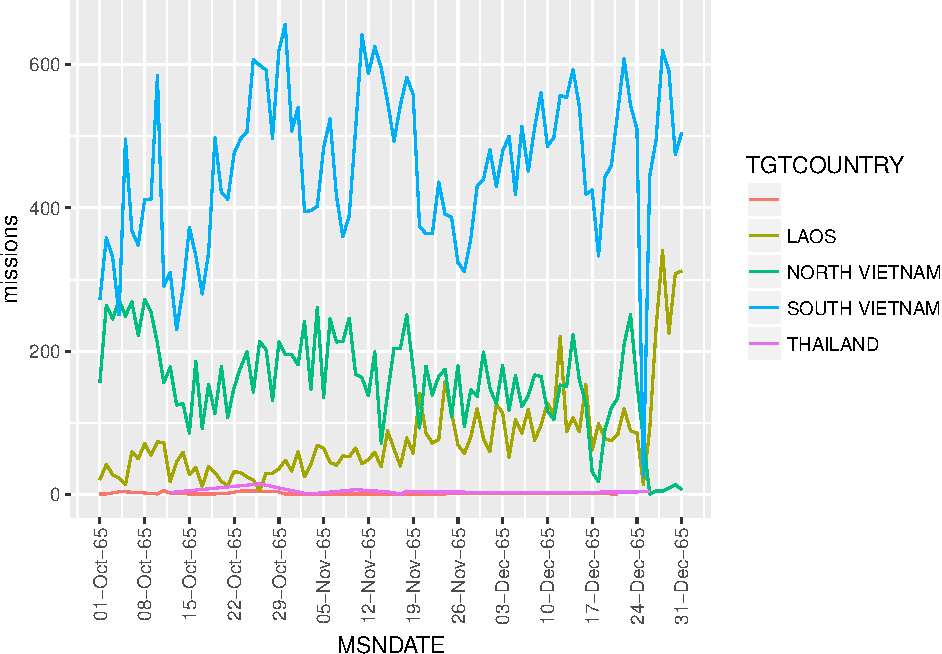
\includegraphics{bookdown-demo_files/figure-latex/unnamed-chunk-36-1.pdf}

\section{Line: Chinese Activity by
Location}\label{line-chinese-activity-by-location}

Change the look of the chart of Chinese government activity.

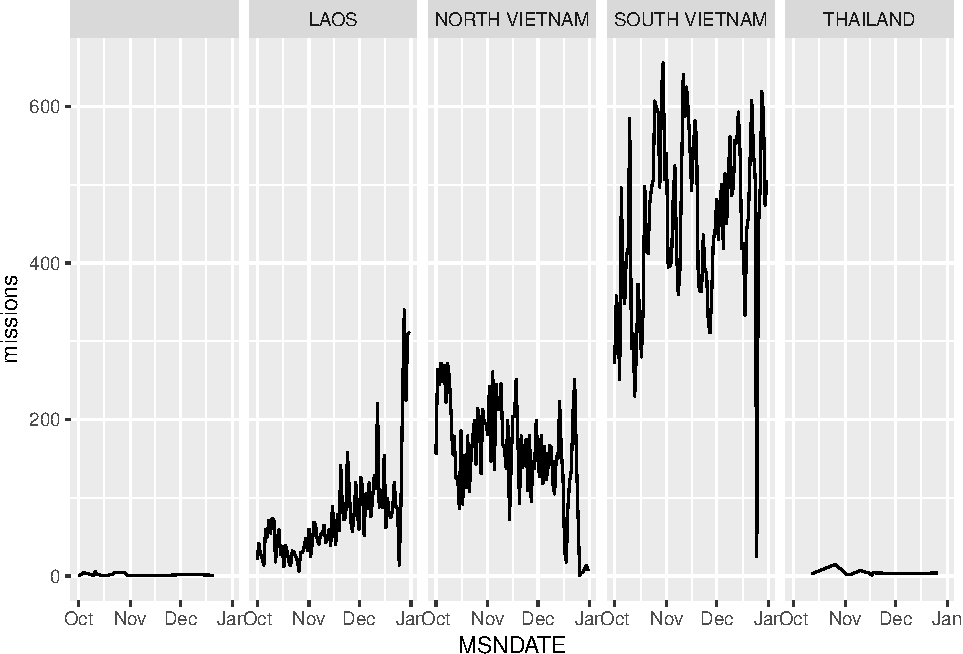
\includegraphics{bookdown-demo_files/figure-latex/unnamed-chunk-37-1.pdf}

\section{Bar: Events by Geographic
Location}\label{bar-events-by-geographic-location}

Hint: \emph{filter()}

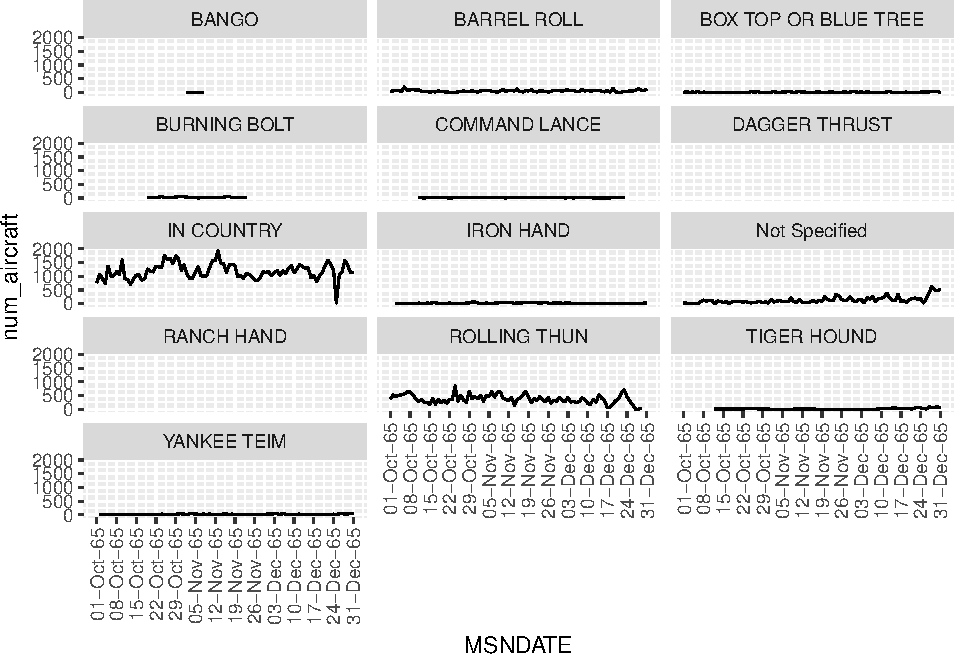
\includegraphics{bookdown-demo_files/figure-latex/unnamed-chunk-38-1.pdf}

\chapter{Exercise Solutions}\label{exercise-solutions}

\section{Change the Look Exercise}\label{change-the-look-exercise-1}

\begin{Shaded}
\begin{Highlighting}[]
\KeywordTok{ggplot}\NormalTok{(subsahara_jan17, }\KeywordTok{aes}\NormalTok{(}\DataTypeTok{x =} \NormalTok{QuadClass)) +}
\StringTok{  }\KeywordTok{geom_bar}\NormalTok{(}\DataTypeTok{fill =} \StringTok{"lightblue"}\NormalTok{, }\DataTypeTok{colour =} \StringTok{"darkblue"}\NormalTok{, }\DataTypeTok{width =} \NormalTok{.}\DecValTok{5}\NormalTok{) +}
\StringTok{  }\KeywordTok{xlab}\NormalTok{(}\StringTok{"Quad Class of the Events"}\NormalTok{) +}
\StringTok{  }\KeywordTok{theme}\NormalTok{(}\DataTypeTok{axis.title.y =} \KeywordTok{element_blank}\NormalTok{()) +}
\StringTok{  }\KeywordTok{ggtitle}\NormalTok{(}\StringTok{"Number of Events by Quad Class"}\NormalTok{) +}
\StringTok{  }\KeywordTok{theme}\NormalTok{(}\DataTypeTok{axis.title.x =} \KeywordTok{element_text}\NormalTok{(}\DataTypeTok{color =} \StringTok{'blue'}\NormalTok{)) +}
\StringTok{  }\KeywordTok{theme}\NormalTok{(}\DataTypeTok{plot.title =} \KeywordTok{element_text}\NormalTok{(}\DataTypeTok{size =} \DecValTok{20}\NormalTok{))}
\end{Highlighting}
\end{Shaded}

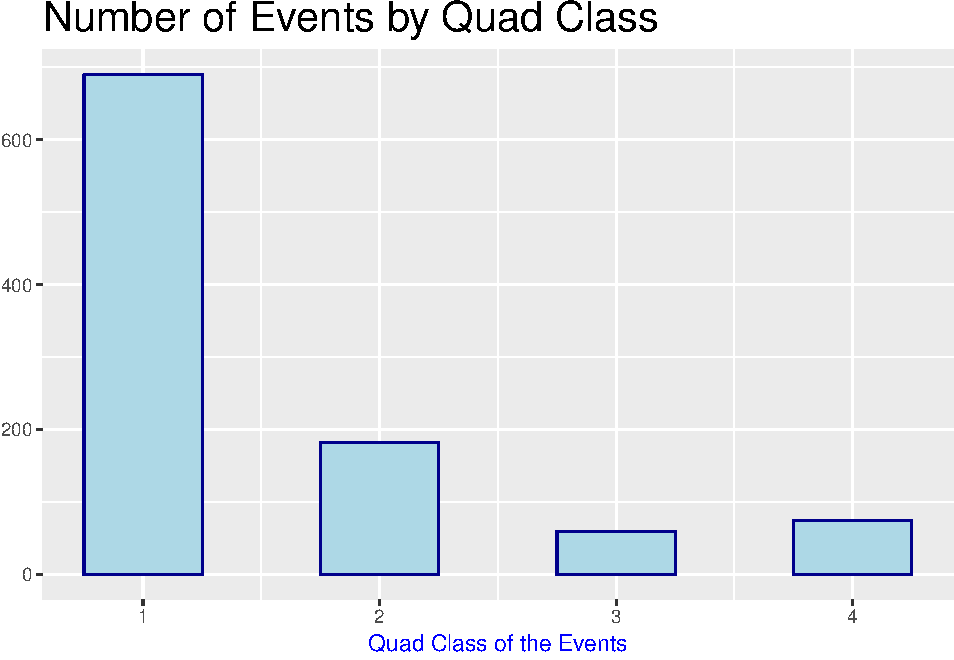
\includegraphics{bookdown-demo_files/figure-latex/unnamed-chunk-40-1.pdf}

\section{PE Part 1}\label{pe-part-1}

\begin{Shaded}
\begin{Highlighting}[]
\NormalTok{subsahara_jan17$EventBaseCode <-}\StringTok{ }\KeywordTok{as.factor}\NormalTok{(subsahara_jan17$EventBaseCode)}
\KeywordTok{ggplot}\NormalTok{(subsahara_jan17, }\KeywordTok{aes}\NormalTok{(}\DataTypeTok{x =} \NormalTok{EventBaseCode)) +}
\StringTok{  }\KeywordTok{geom_bar}\NormalTok{(}\DataTypeTok{fill =} \StringTok{"red"}\NormalTok{, }\DataTypeTok{colour =} \StringTok{"black"}\NormalTok{, }\DataTypeTok{width =} \NormalTok{.}\DecValTok{5}\NormalTok{) +}
\StringTok{  }\KeywordTok{theme}\NormalTok{(}\DataTypeTok{axis.text.x =} \KeywordTok{element_text}\NormalTok{(}\DataTypeTok{angle =} \DecValTok{90}\NormalTok{, }\DataTypeTok{hjust =} \NormalTok{.}\DecValTok{5}\NormalTok{, }\DataTypeTok{vjust =} \NormalTok{.}\DecValTok{5}\NormalTok{)) +}
\StringTok{  }\KeywordTok{xlab}\NormalTok{(}\StringTok{"Event Code"}\NormalTok{) +}\StringTok{ }
\StringTok{  }\KeywordTok{theme}\NormalTok{(}\DataTypeTok{axis.title.y =} \KeywordTok{element_blank}\NormalTok{()) +}\StringTok{  }
\StringTok{  }\KeywordTok{ggtitle}\NormalTok{(}\StringTok{"Number of Events by Event Code"}\NormalTok{)}
\end{Highlighting}
\end{Shaded}

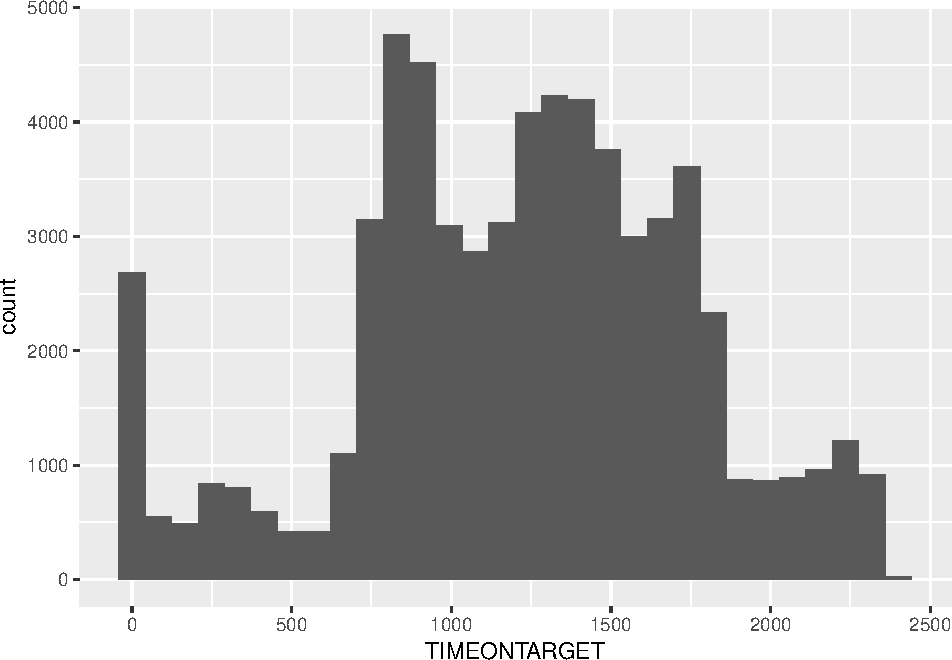
\includegraphics{bookdown-demo_files/figure-latex/unnamed-chunk-41-1.pdf}

\section{PE Part 2}\label{pe-part-2}

\begin{Shaded}
\begin{Highlighting}[]
\KeywordTok{ggplot}\NormalTok{(china_2weeks, }\KeywordTok{aes}\NormalTok{(}\DataTypeTok{x =} \KeywordTok{as.Date}\NormalTok{(days), }\DataTypeTok{y =} \NormalTok{n, }\DataTypeTok{color =} \NormalTok{country))+}
\StringTok{  }\KeywordTok{geom_line}\NormalTok{(}\DataTypeTok{size =} \DecValTok{1}\NormalTok{) +}
\StringTok{  }\KeywordTok{ggtitle}\NormalTok{(}\StringTok{"Events Involving the Chinese Government in 3 Countries"}\NormalTok{)+}
\StringTok{  }\KeywordTok{theme}\NormalTok{(}\DataTypeTok{plot.title =} \KeywordTok{element_text}\NormalTok{(}\DataTypeTok{hjust =} \NormalTok{.}\DecValTok{5}\NormalTok{)) +}\StringTok{  }\CommentTok{#Center the plot title}
\StringTok{  }\KeywordTok{theme}\NormalTok{(}\DataTypeTok{axis.title.y =} \KeywordTok{element_blank}\NormalTok{()) +}
\StringTok{  }\KeywordTok{theme}\NormalTok{(}\DataTypeTok{axis.title.x =} \KeywordTok{element_blank}\NormalTok{()) +}
\StringTok{  }\KeywordTok{scale_x_date}\NormalTok{(}\DataTypeTok{breaks =} \NormalTok{dailybreaks) +}
\StringTok{  }\KeywordTok{theme}\NormalTok{(}\DataTypeTok{axis.text.x =} \KeywordTok{element_text}\NormalTok{(}\DataTypeTok{angle =} \DecValTok{90}\NormalTok{, }\DataTypeTok{hjust =} \DecValTok{1}\NormalTok{, }\DataTypeTok{vjust =} \DecValTok{0}\NormalTok{)) +}\StringTok{  }\CommentTok{#change angle of axis text}
\StringTok{  }\KeywordTok{theme}\NormalTok{(}\DataTypeTok{legend.position =} \StringTok{"top"}\NormalTok{)+}\StringTok{  }\CommentTok{#legend to top of chart}
\StringTok{  }\KeywordTok{labs}\NormalTok{(}\DataTypeTok{color =} \StringTok{"Location of Activity"}\NormalTok{) +}
\StringTok{  }\KeywordTok{geom_point}\NormalTok{(}\DataTypeTok{shape =} \DecValTok{18}\NormalTok{, }\DataTypeTok{size =} \DecValTok{4}\NormalTok{) +}
\StringTok{  }\KeywordTok{scale_color_brewer}\NormalTok{(}\DataTypeTok{palette =} \StringTok{"Set1"}\NormalTok{, }\DataTypeTok{labels =} \KeywordTok{c}\NormalTok{(}\StringTok{"Nigeria"}\NormalTok{,}\StringTok{"Zambia"}\NormalTok{,}\StringTok{"Zimbabwe"}\NormalTok{))}
\end{Highlighting}
\end{Shaded}

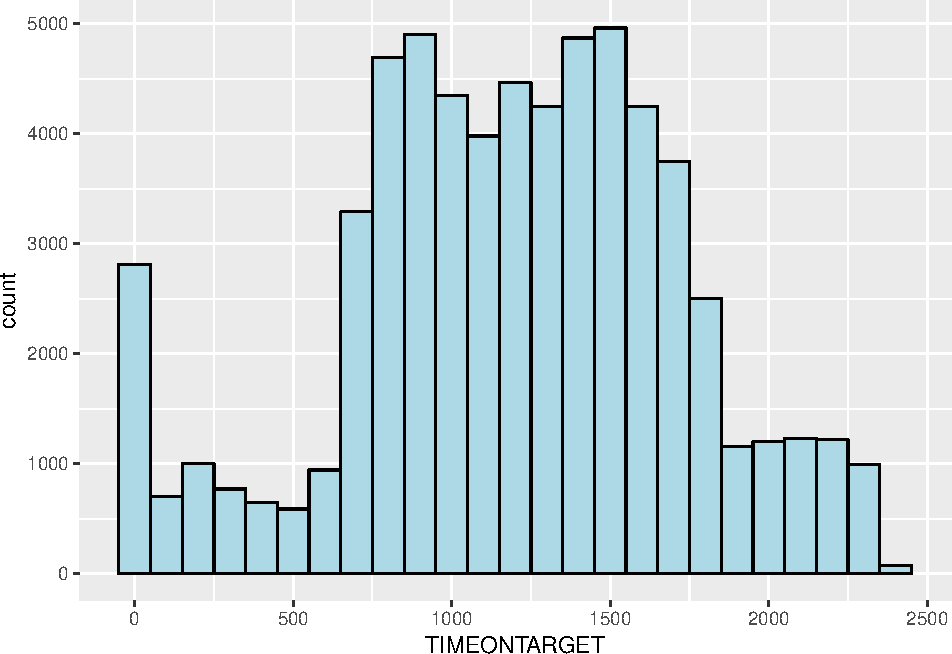
\includegraphics{bookdown-demo_files/figure-latex/unnamed-chunk-42-1.pdf}

\section{PE Part 3}\label{pe-part-3}

\begin{Shaded}
\begin{Highlighting}[]
\NormalTok{sub51 <-}\StringTok{ }\NormalTok{dplyr::}\KeywordTok{filter}\NormalTok{(subsahara_jan17, EventBaseCode ==}\StringTok{ }\DecValTok{51}\NormalTok{)}
\KeywordTok{ggplot}\NormalTok{(sub51, }\KeywordTok{aes}\NormalTok{(}\DataTypeTok{x=} \NormalTok{EventBaseCode, }\DataTypeTok{fill =} \NormalTok{ActionGeo_ADM1Code))+}
\StringTok{  }\KeywordTok{geom_bar}\NormalTok{(}\DataTypeTok{position =} \StringTok{'dodge'}\NormalTok{, }\DataTypeTok{color =} \StringTok{"black"}\NormalTok{)+}
\StringTok{  }\KeywordTok{ggtitle}\NormalTok{(}\StringTok{"Number of Events by Action Geographic Location}\CharTok{\textbackslash{}n}\StringTok{ for Event Code with the Most Events"}\NormalTok{) +}
\StringTok{  }\KeywordTok{xlab}\NormalTok{(}\StringTok{"Event Code"}\NormalTok{) +}
\StringTok{  }\KeywordTok{labs}\NormalTok{(}\DataTypeTok{fill =} \StringTok{"Geographic Location"}\NormalTok{)+}
\StringTok{  }\KeywordTok{scale_fill_brewer}\NormalTok{(}\DataTypeTok{palette =} \StringTok{"Set3"}\NormalTok{)}
\end{Highlighting}
\end{Shaded}

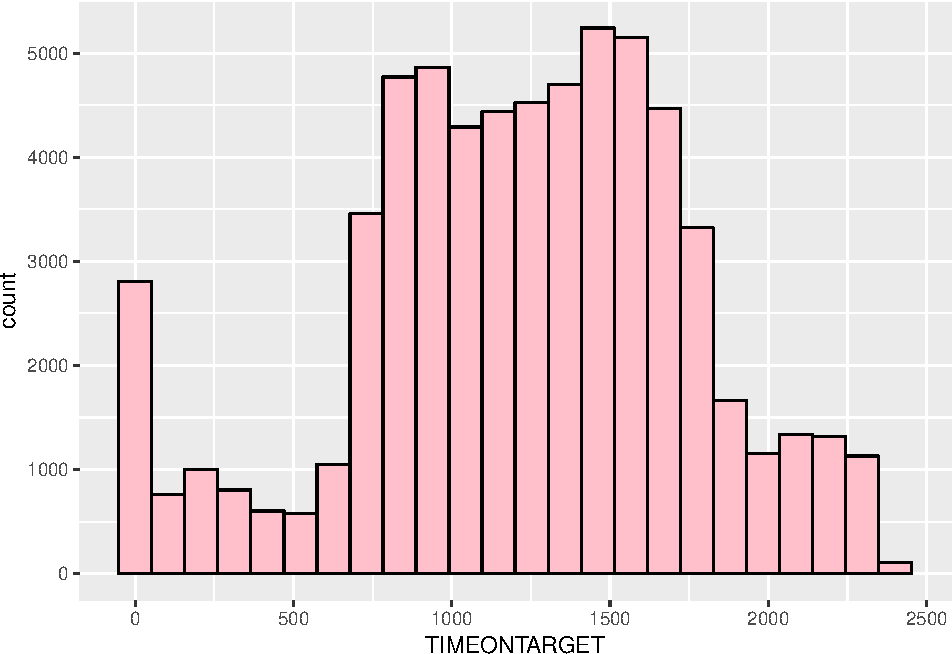
\includegraphics{bookdown-demo_files/figure-latex/unnamed-chunk-43-1.pdf}


\end{document}
